Figure~\ref{fig:hw_ballbeam_compensator_in_design_1} shows the Bode plot of the plant $P_{in}(s)$ together with the design specification on tracking and noise attenuation.
%
\begin{figure}[H]
   \centering
   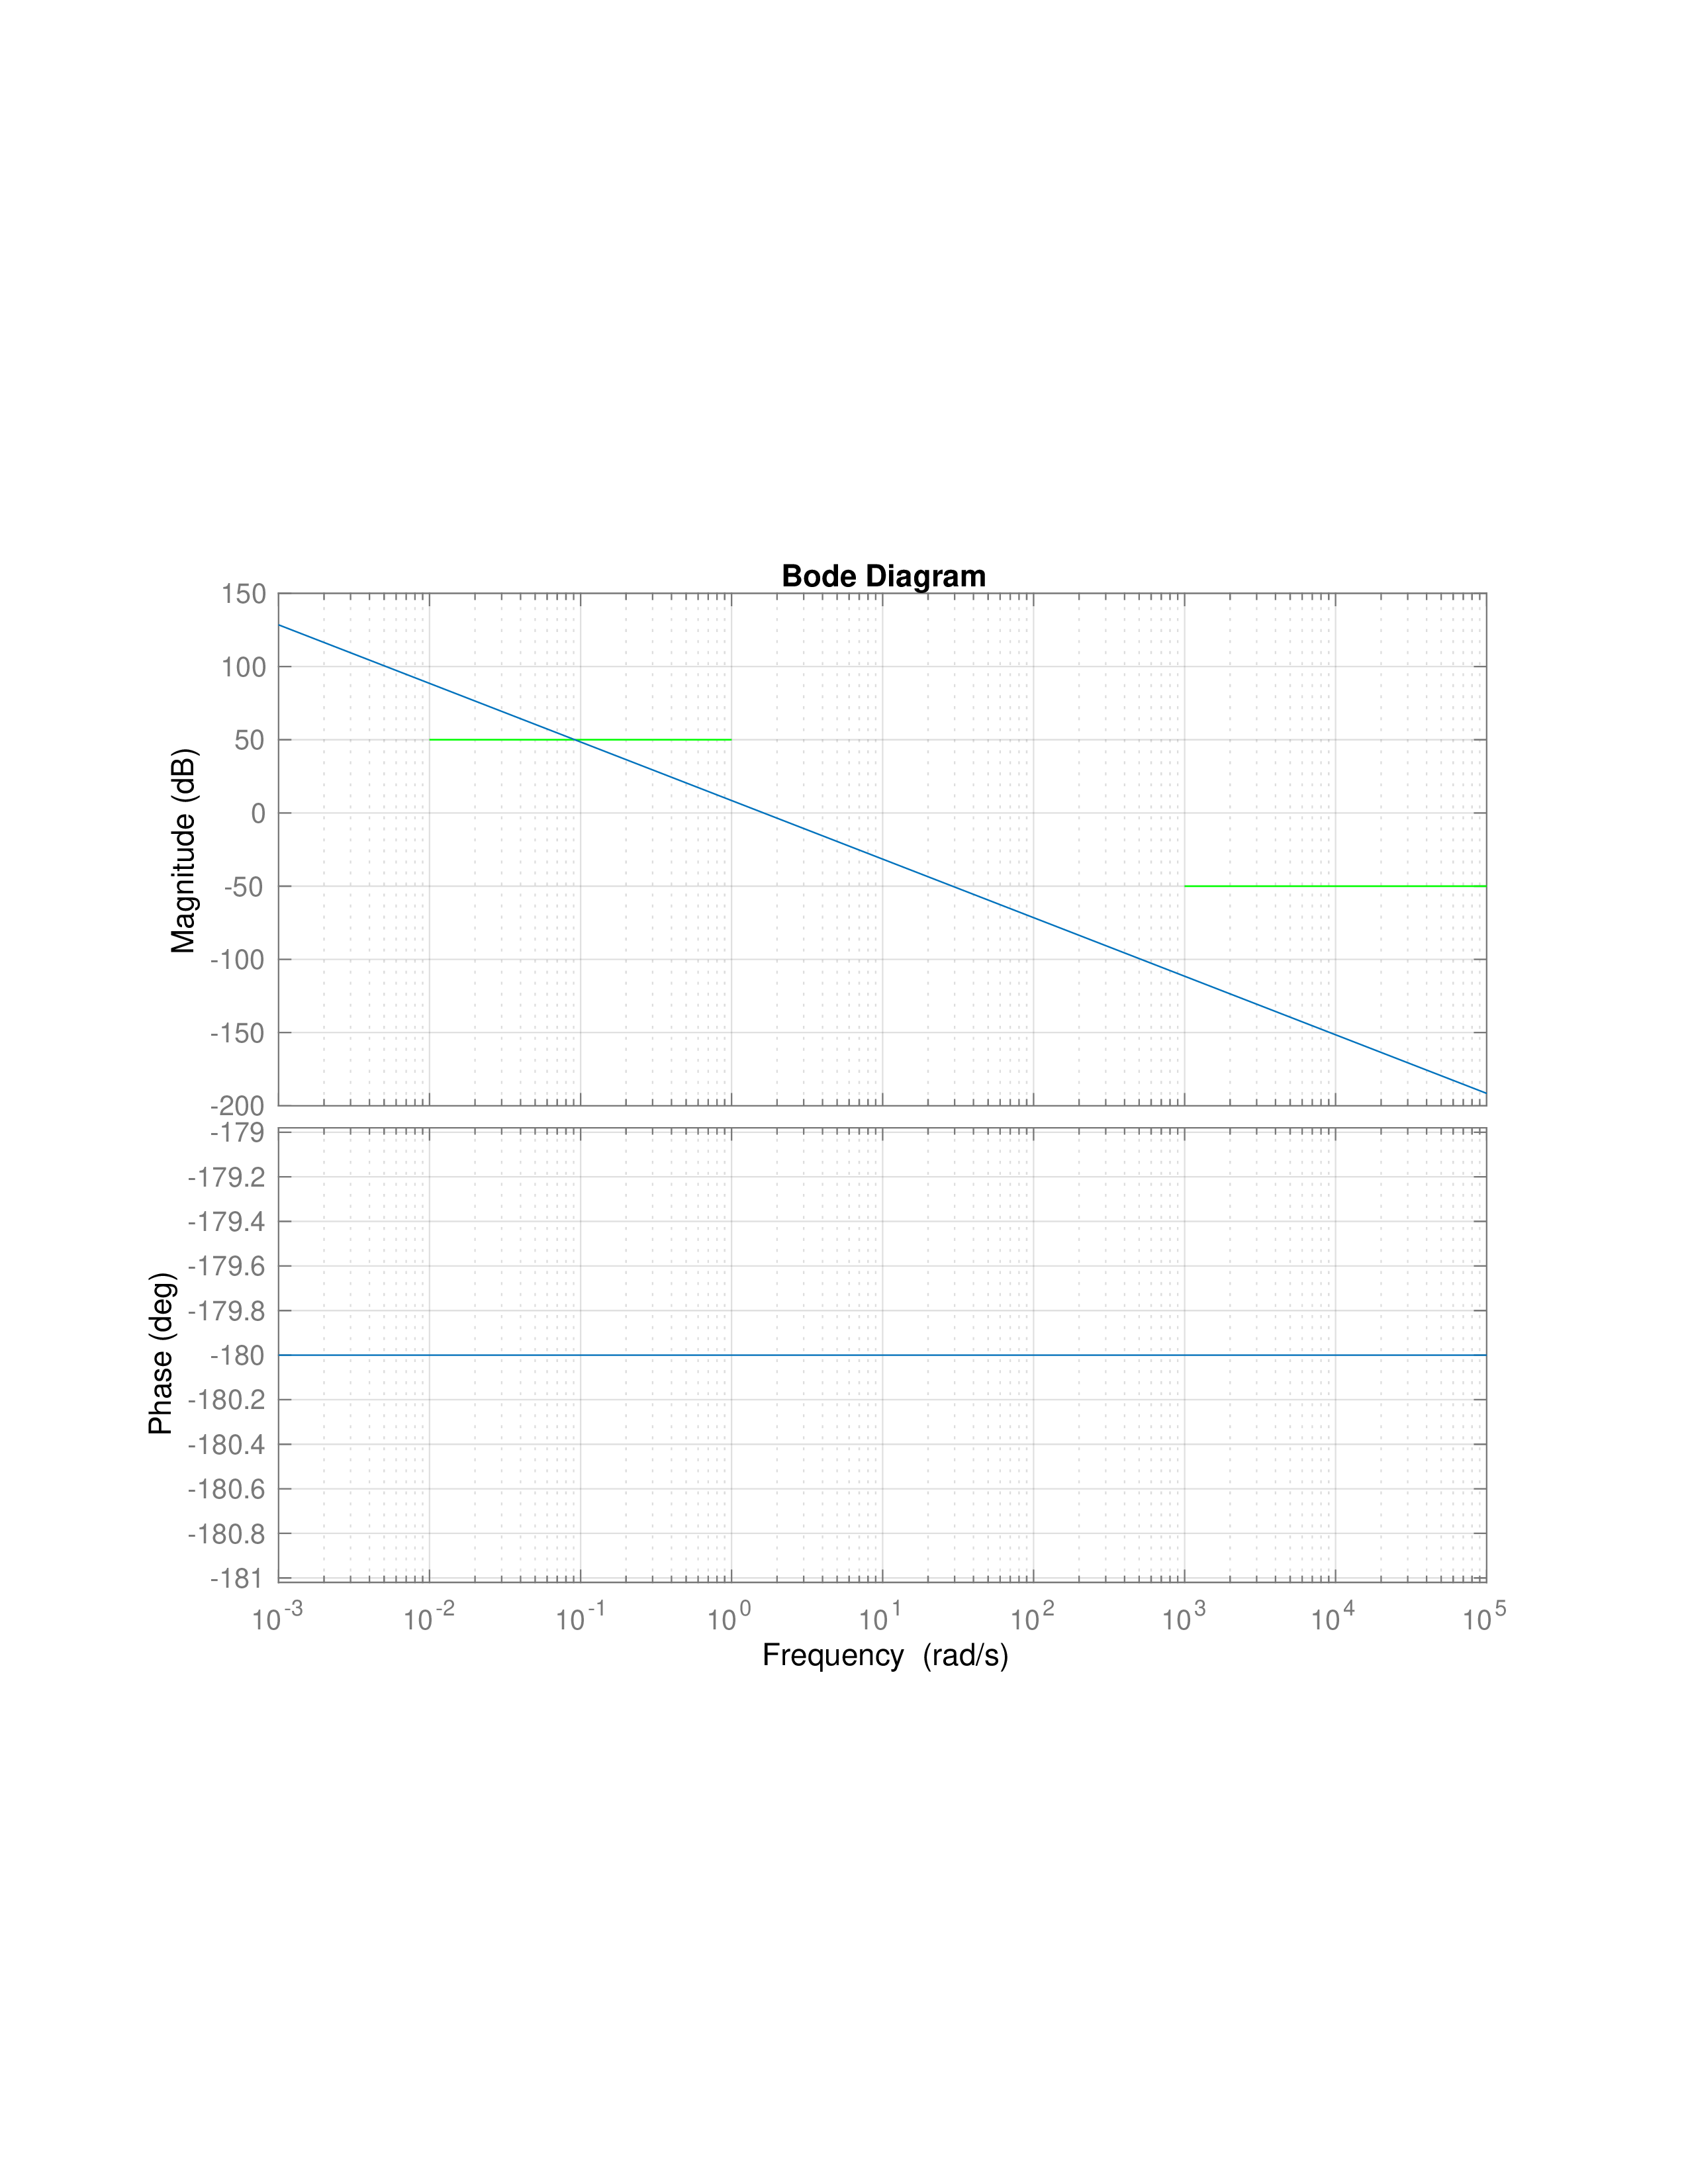
\includegraphics[width=0.95\textwidth]{6_design_studies/figures/hw_ballbeam_compensator_in_design_1.pdf}
   \caption{The Bode plot for the inner loop plant in HW~\ref{hw:ballbeam}.\ref{chap:loopshaping_design}, together with the design specification.}
   \label{fig:hw_ballbeam_compensator_in_design_1}
\end{figure}
The first step is to add a proportional gain so that the open loop response below $\omega_r=1$~radians/sec is above $20\log_{10}\gamma_r^{-1} = 50$~dB.  Figure~\ref{fig:hw_ballbeam_compensator_in_design_2} shows the corresponding Bode plot for a proportional gain of $k_p=150$.
\begin{figure}[H]
   \centering
   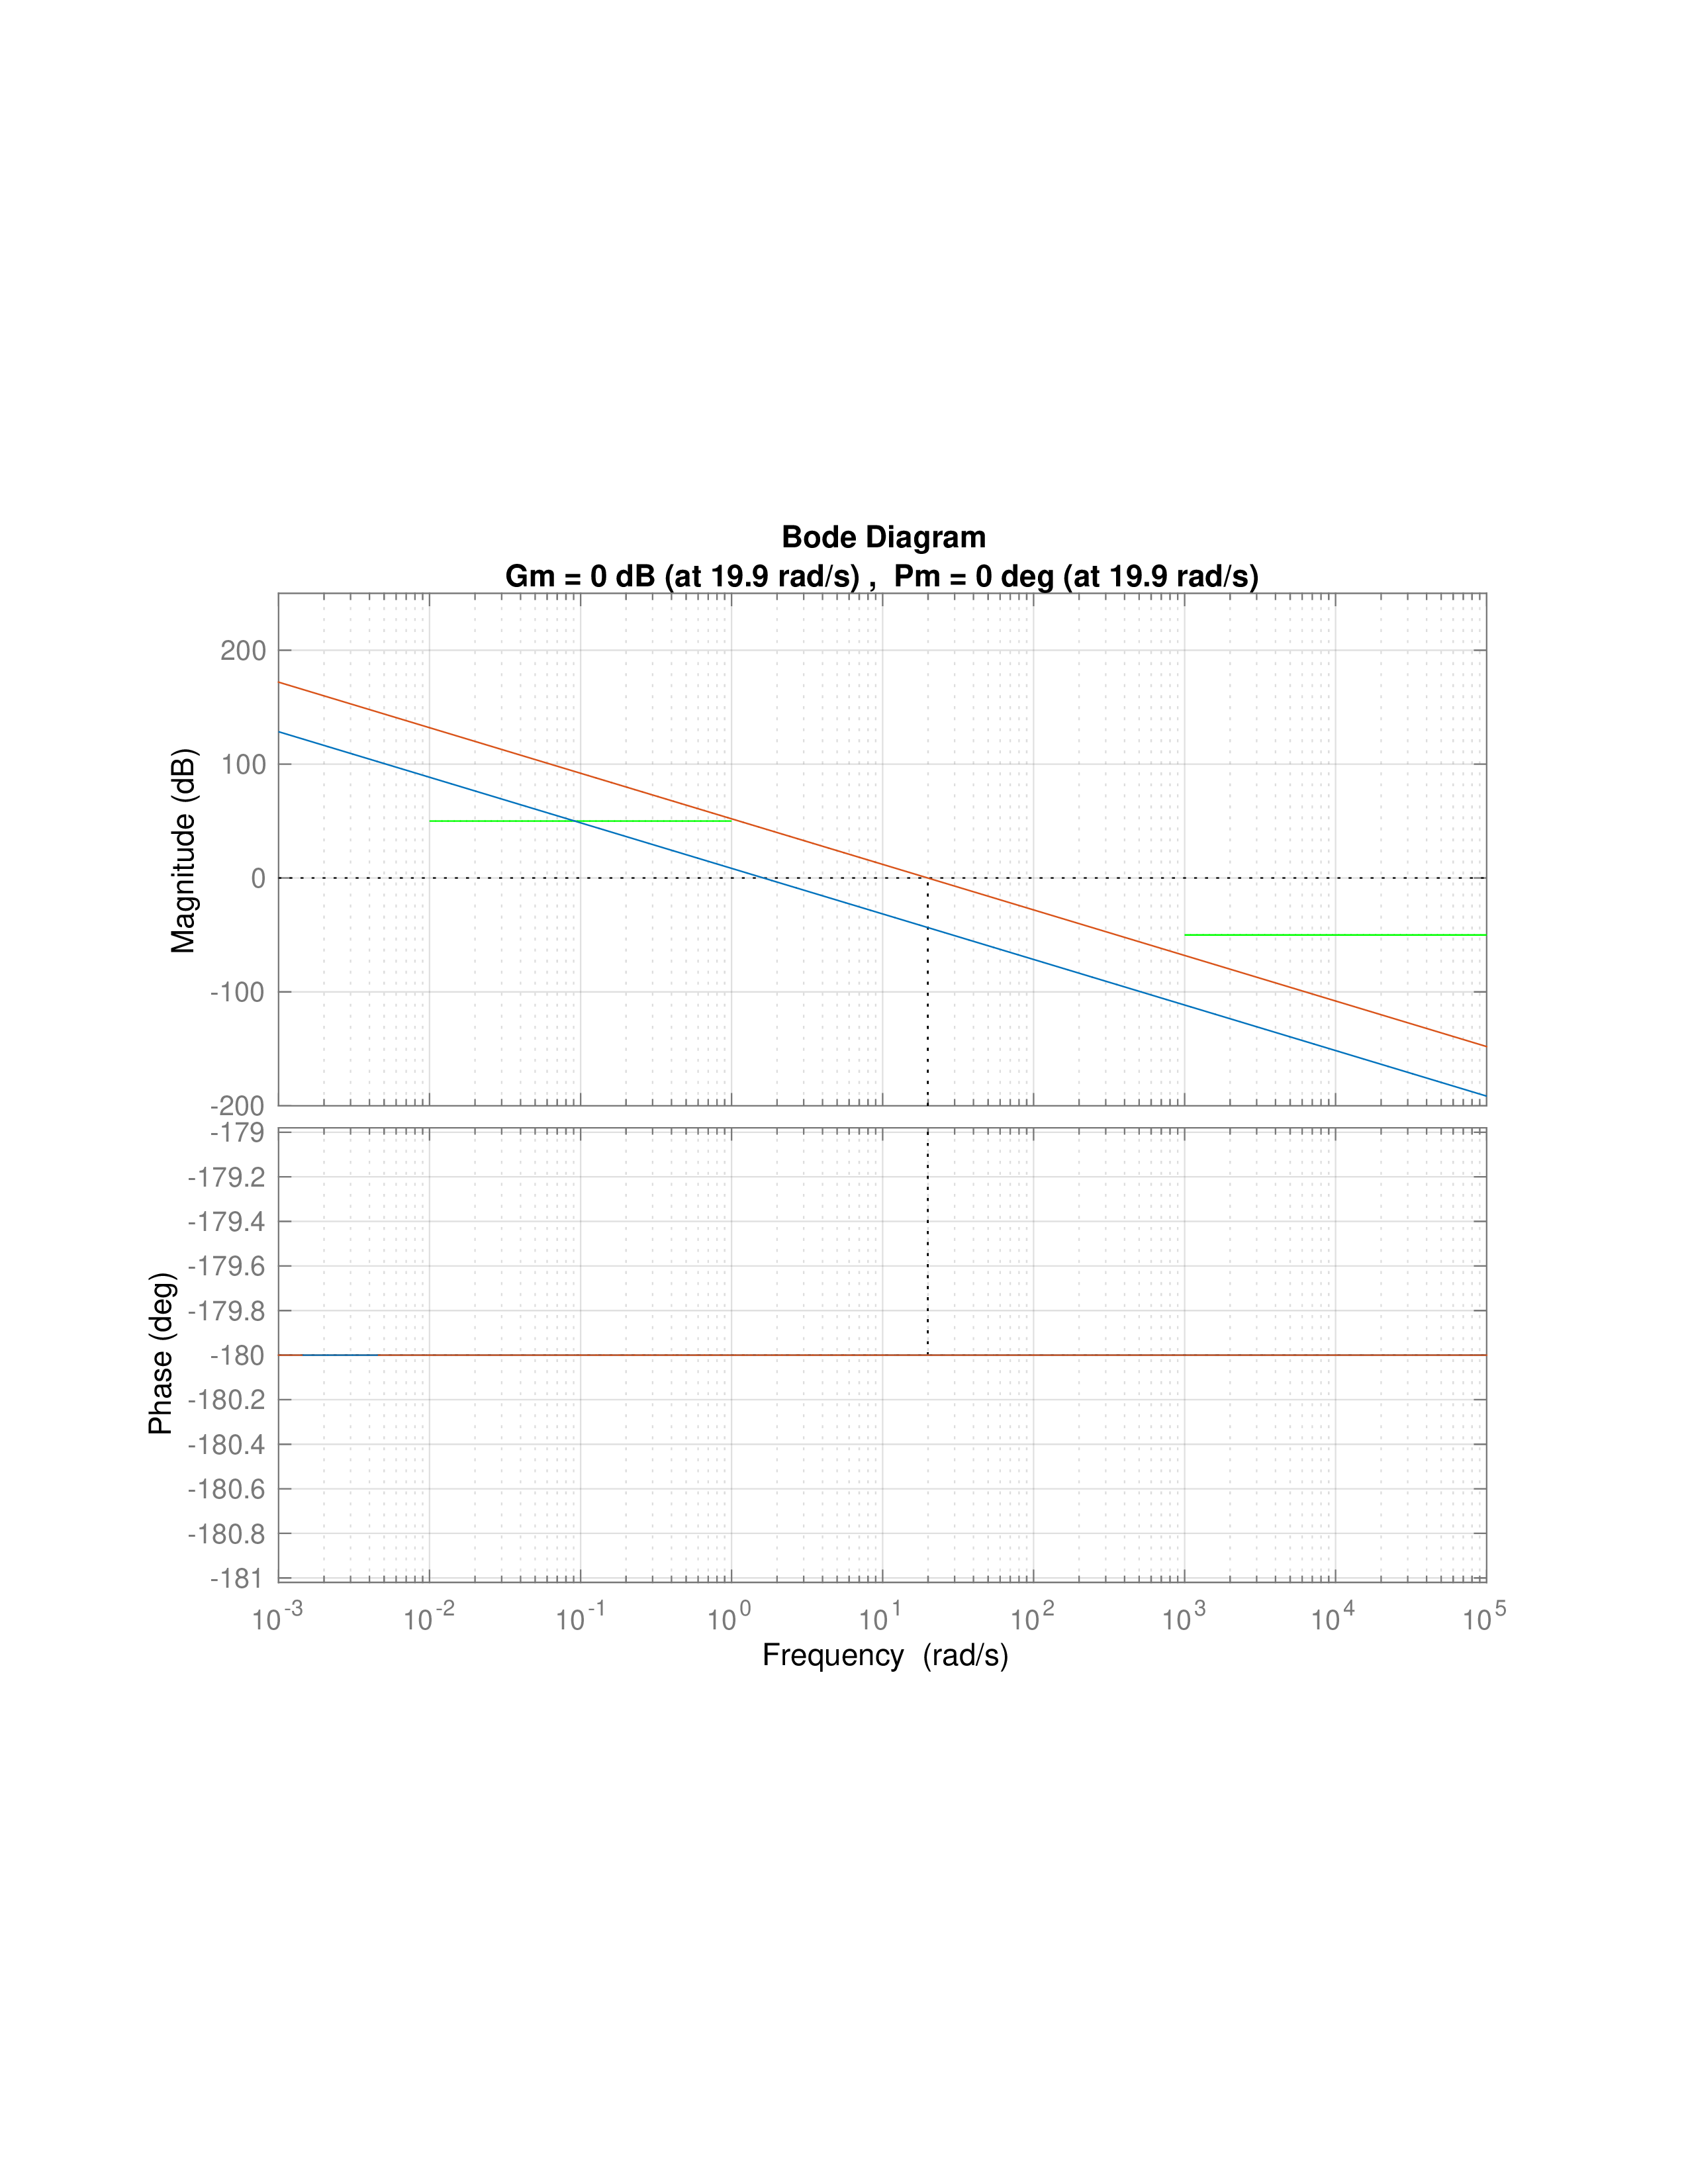
\includegraphics[width=0.95\textwidth]{6_design_studies/figures/hw_ballbeam_compensator_in_design_2.pdf}
   \caption{The Bode plot for the inner loop plant in HW~\ref{hw:ballbeam}.\ref{chap:loopshaping_design}, with proportional gain.}
   \label{fig:hw_ballbeam_compensator_in_design_2}
\end{figure}
To stabilize the system, a phase lead compensator needs to be added around the cross over frequency.  Figure~\ref{fig:hw_ballbeam_compensator_in_design_3} shows the addition of the phase lead filter
\[
C_{lead} = \frac{15(s+\frac{40}{\sqrt{15}})}{(s+\frac{40}{\sqrt{15}})},
\]
which has a phase margin of $PM=61$~degrees.
\begin{figure}[H]
   \centering
   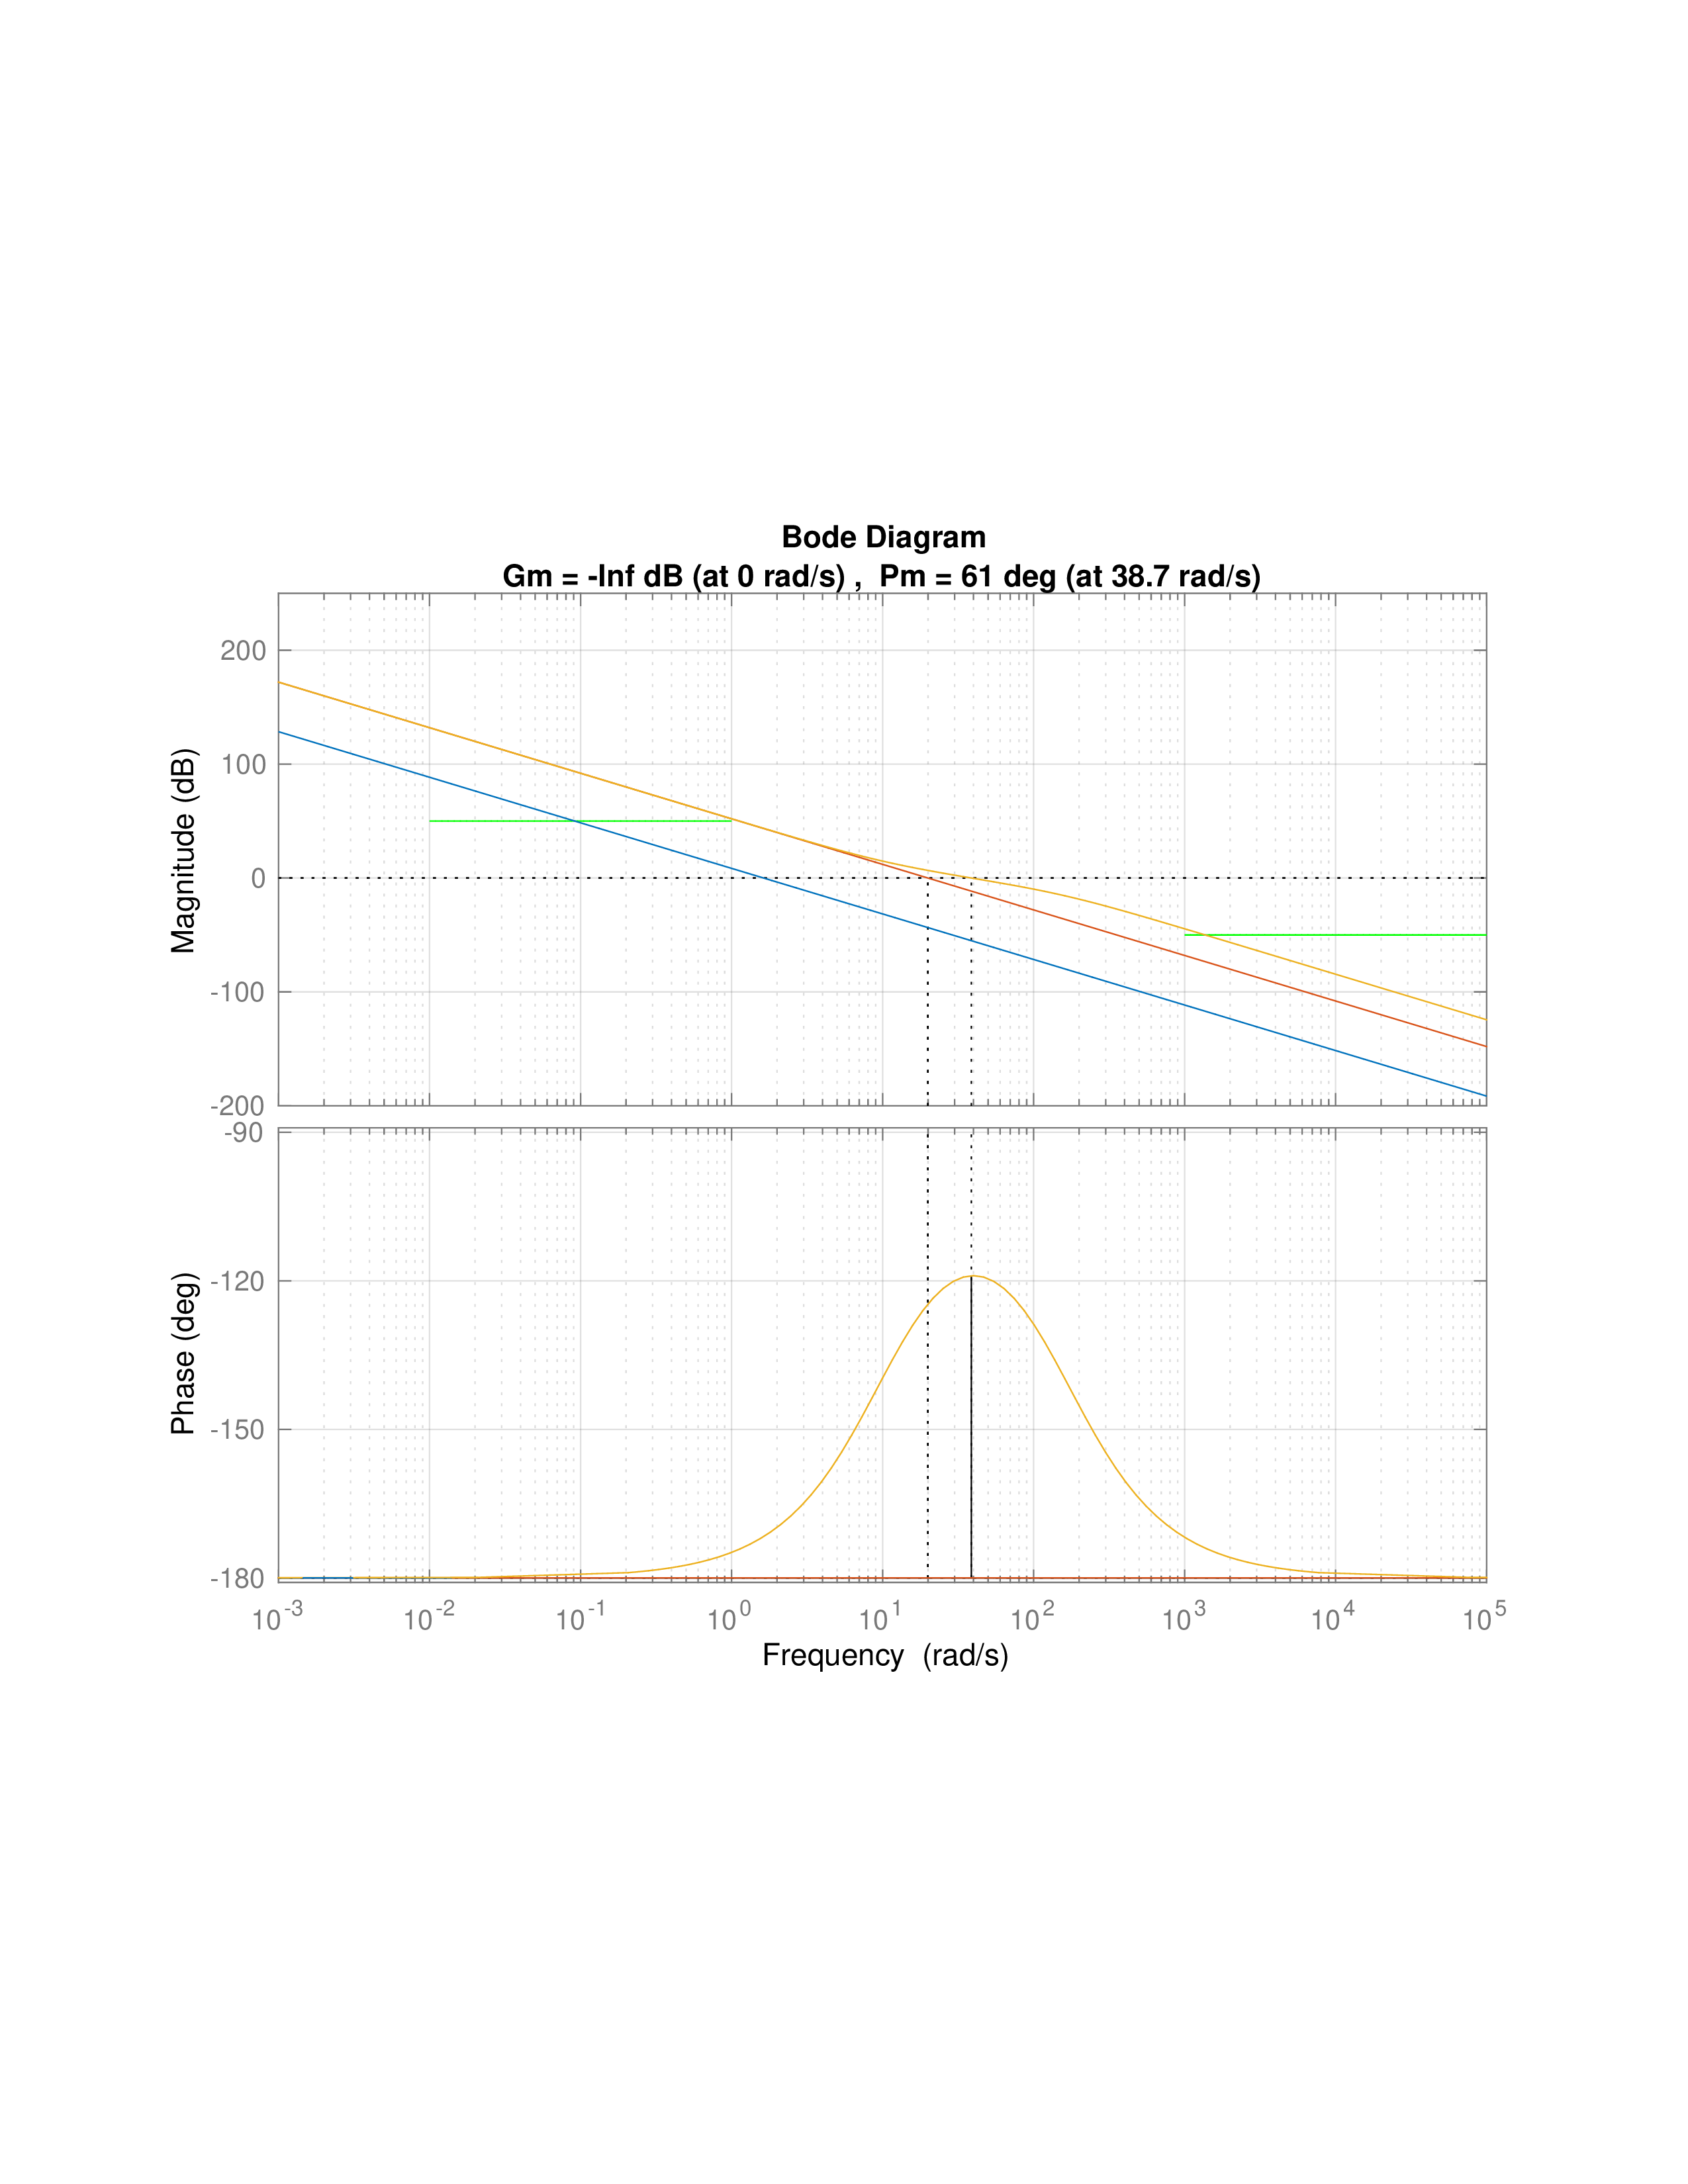
\includegraphics[width=0.95\textwidth]{6_design_studies/figures/hw_ballbeam_compensator_in_design_3.pdf}
   \caption{The Bode plot for the inner loop system in HW~\ref{hw:ballbeam}.\ref{chap:loopshaping_design}, with proportional gain and phase lead compensation.}
   \label{fig:hw_ballbeam_compensator_in_design_3}
\end{figure}
The noise specification is met by adding the low pass filter
\[
C_{lpf} = \frac{500}{s+500}
\]
as shown in Figure~\ref{fig:hw_ballbeam_compensator_in_design_4}.
\begin{figure}[H]
   \centering
   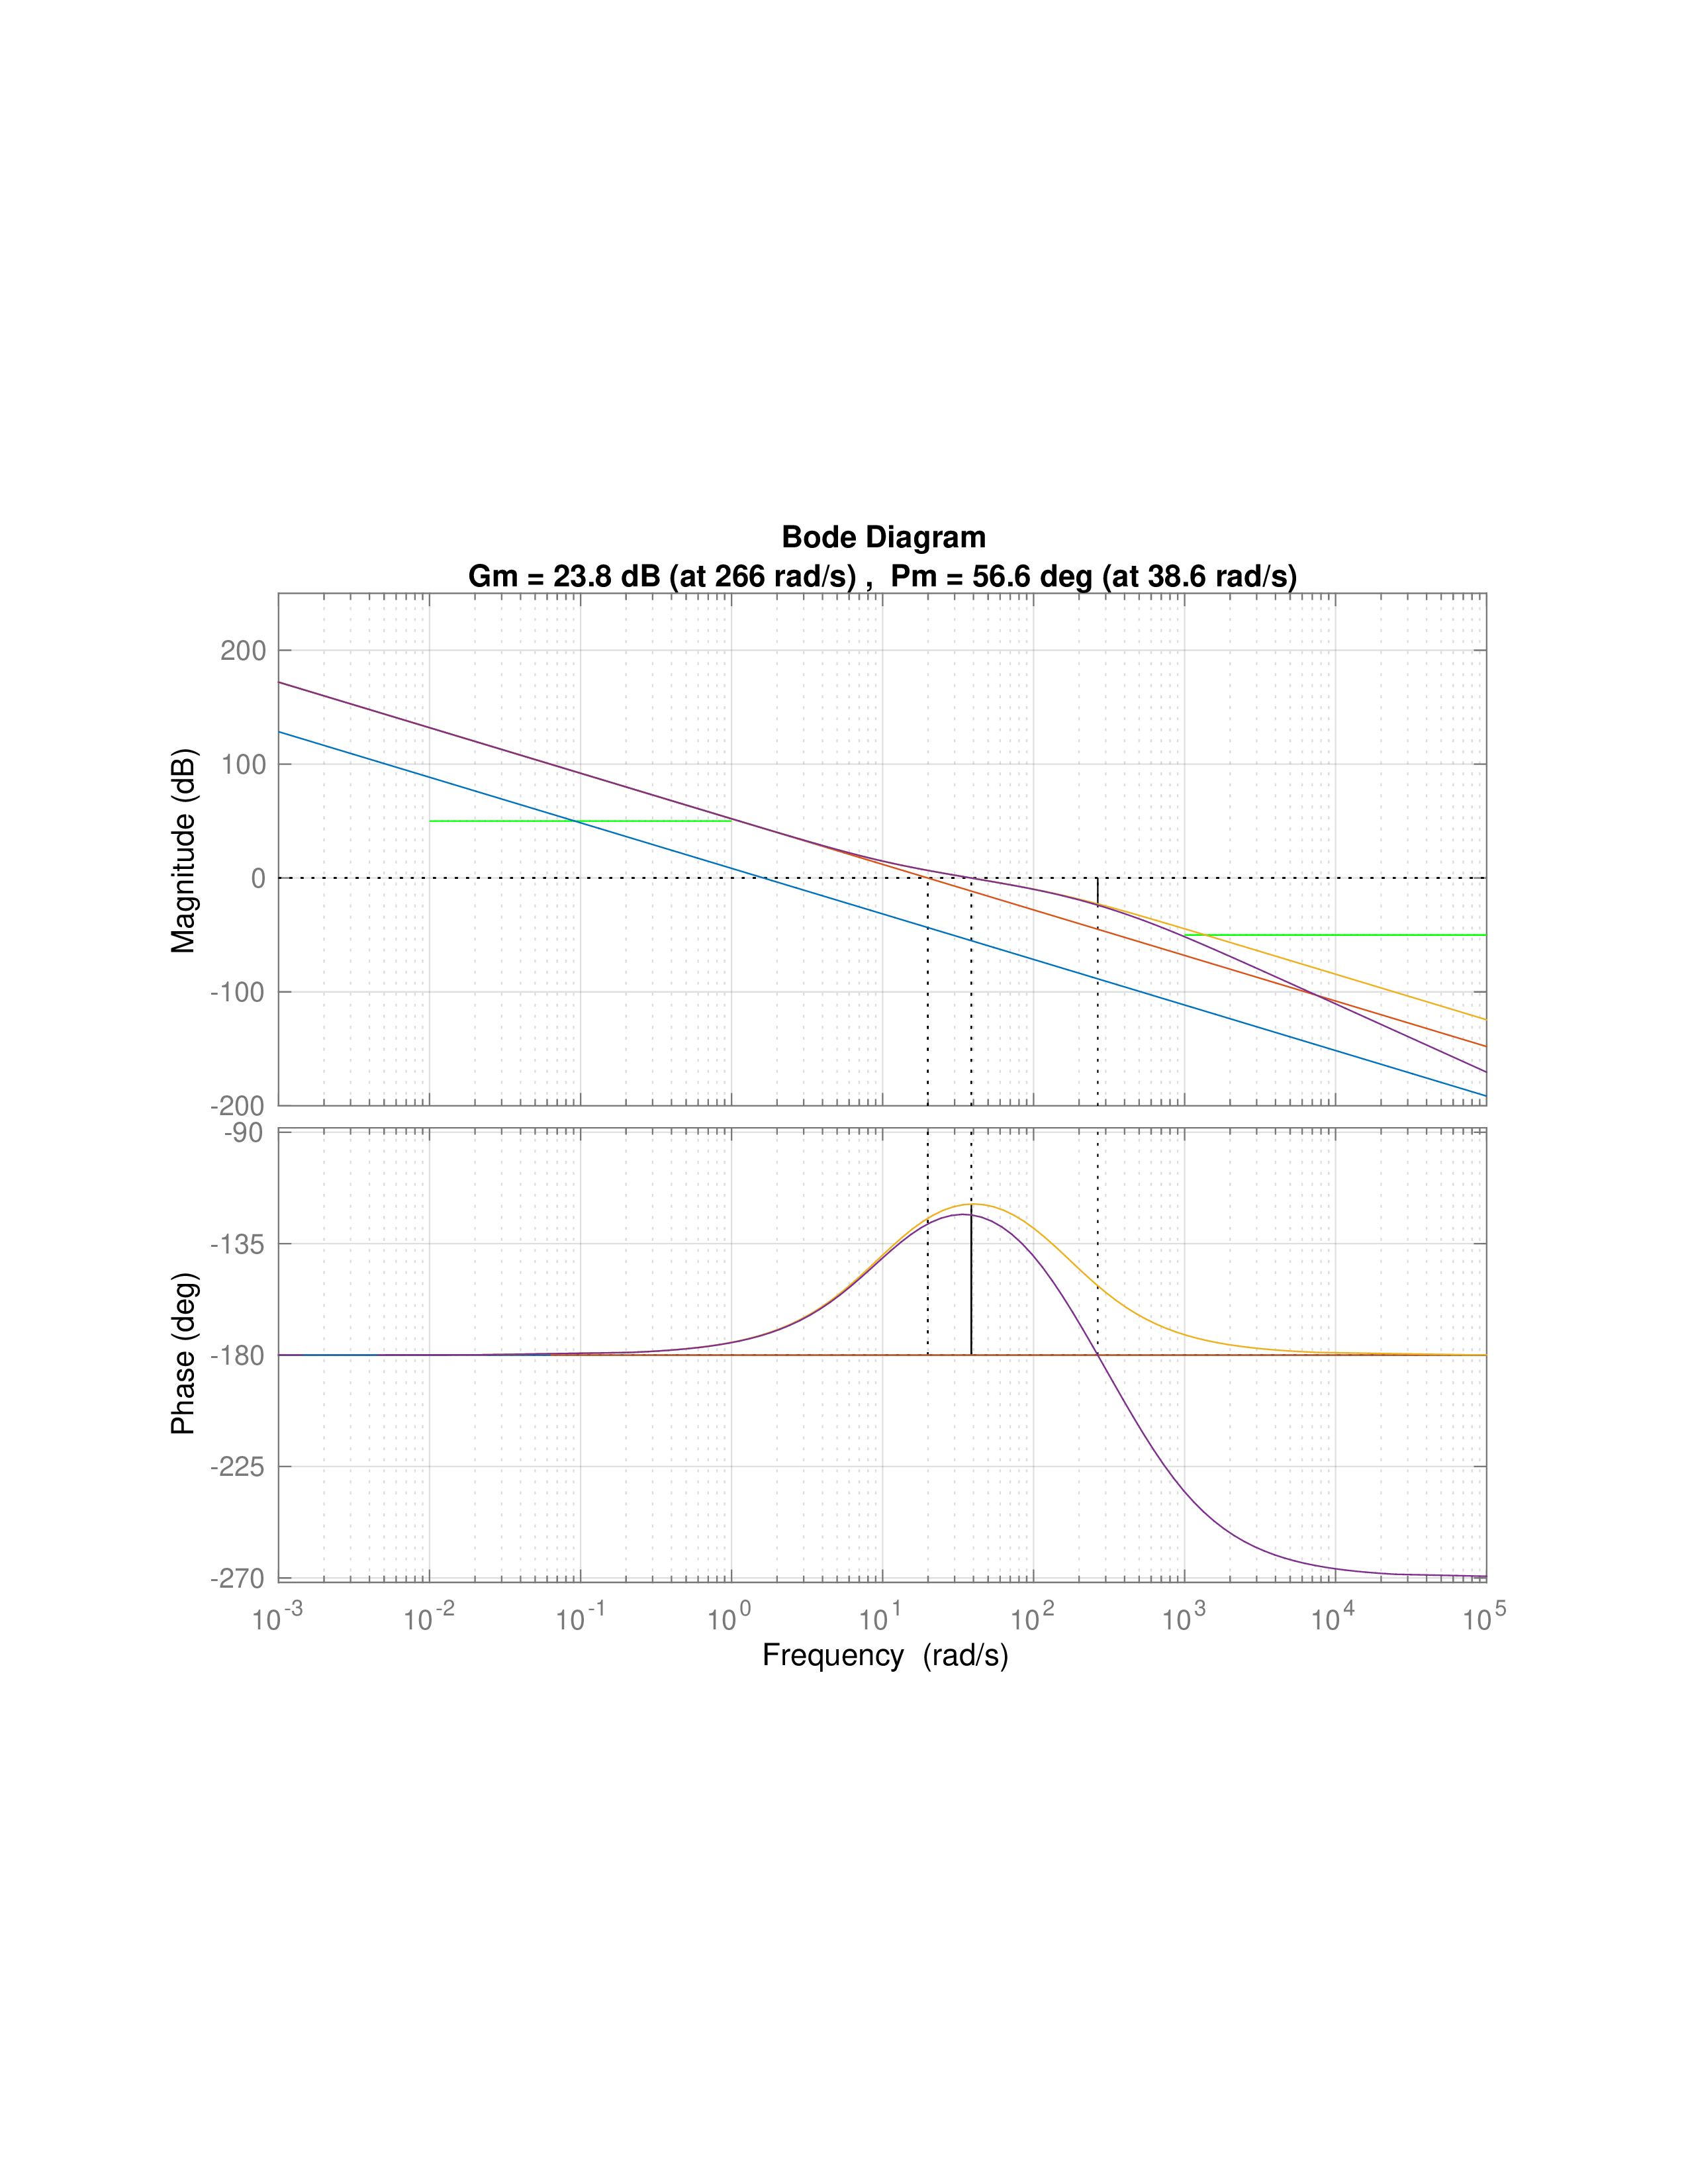
\includegraphics[width=0.95\textwidth]{6_design_studies/figures/hw_ballbeam_compensator_in_design_4.pdf}
   \caption{The Bode plot for the inner loop system in HW~\ref{hw:ballbeam}.\ref{chap:loopshaping_design}, with proportional gain, phase lead compensation, and a low pass filter.}
   \label{fig:hw_ballbeam_compensator_in_design_4}
\end{figure}
The compensator for the inner loop is given by
\[
C_{in}(s) = 150 \left(\frac{15(s+\frac{40}{\sqrt{15}})}{(s+\frac{40}{\sqrt{15}})}\right)\left(\frac{500}{s+500}\right).
\]
The closed loop response for the inner subsystem
\[
\frac{P_{in}C_{in}}{1+P_{in}C_{in}},
\] 
as well as the unit step response for the output and control signal are all show in Figure~\ref{fig:hw_ballbeam_compensator_in_design_5}.
\begin{figure}[H]
   \centering
   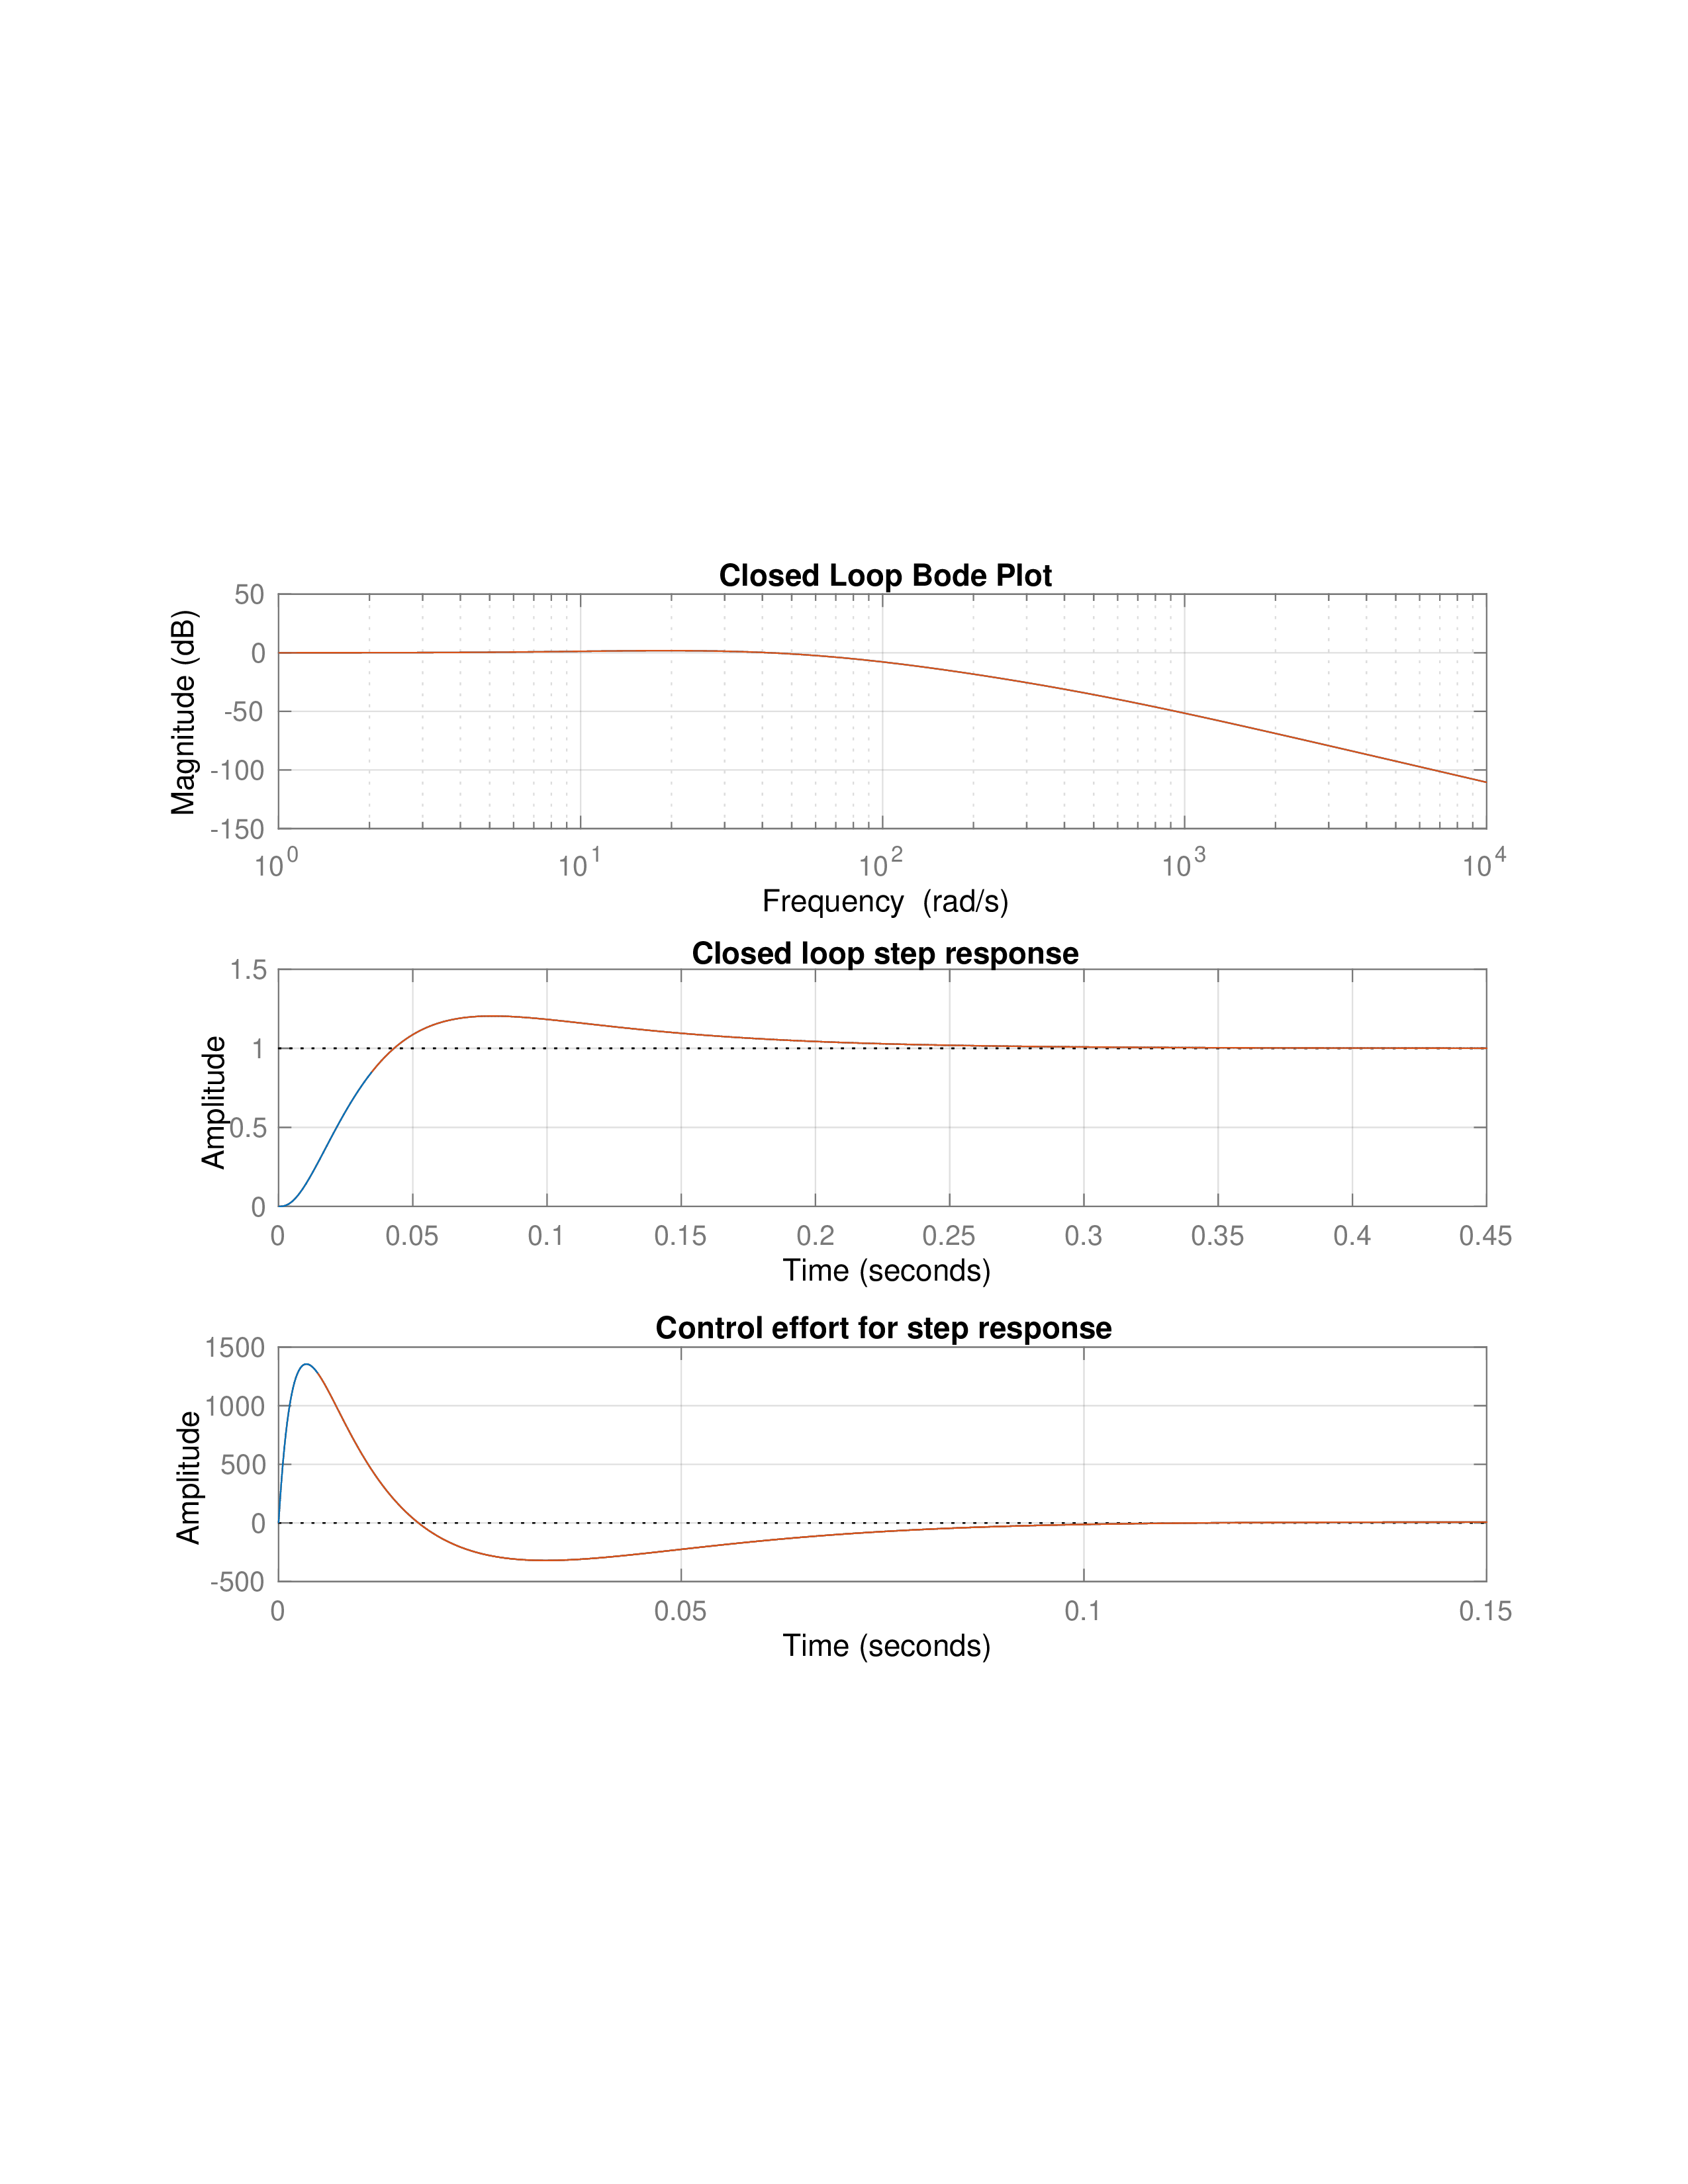
\includegraphics[width=0.95\textwidth]{6_design_studies/figures/hw_ballbeam_compensator_in_design_5.pdf}
   \caption{The closed loop bode response, the unit step response for the output, and the unit step response for the input of the inner loop design in HW~\ref{hw:ballbeam}.\ref{chap:loopshaping_design}.}
   \label{fig:hw_ballbeam_compensator_in_design_5}
\end{figure}

The Matlab code used to design the inner loop is shown below.
\begin{lstlisting}
Plant = P_in;

%%%%%%%%%%%%%%%%%%%%%%%%%%%%%%%%%%%%%%%%%%%%%%%%%%%%%%%%%%%
%  Define Design Specifications
%%%%%%%%%%%%%%%%%%%%%%%%%%%%%%%%%%%%%%%%%%%%%%%%%%%%%%%%%%%

%--- general tracking specification ---
    omega_r = 10^0;  % track signals below this frequency
    gamma_r = 10^(-50/20);  % tracking error below this value
    w = logspace(log10(omega_r)-2,log10(omega_r));

%--- noise specification ---
    omega_n = 10^3;  % attenuate noise above this frequency
    gamma_n = 10^(-50/20);   % attenuate noise by this amount
    w = logspace(log10(omega_n),2+log10(omega_n));
    plot(w,20*log10(gamma_n)*ones(size(w)),'g')
        
%%%%%%%%%%%%%%%%%%%%%%%%%%%%%%%%%%%%%%%%%%%%%%%%%%%%%%%%%%%
% Control Design
  C = tf(1,1);
%%%%%%%%%%%%%%%%%%%%%%%%%%%%%%%%%%%%%%%%%%%%%%%%%%%%%%%%%%%

% proportional control: change cross over frequency
     kp = 150;
     C = C*kp;
     
% phase lead: increase PM (stability)
    wmax = 40; % location of maximum frequency bump
    M    = 15; % separation between zero and pole
    Lead =tf(M*[1,wmax/sqrt(M)],[1,wmax*sqrt(M)]);
    C = C*Lead;
    
% low pass filter: decrease gain at high frequency (noise)
     p = 500;
     LPF = tf(p,[1,p]);
     C = C*LPF;
       
%%%%%%%%%%%%%%%%%%%%%%%%%%%%%%%%%%%%%%%%%%%%%%%%%%%%%%%%%
% Convert controller to state space equations 
%%%%%%%%%%%%%%%%%%%%%%%%%%%%%%%%%%%%%%%%%%%%%%%%%%%%%%%%%
[num,den] = tfdata(C,'v');
[P.Ain_C,P.Bin_C,P.Cin_C,P.Din_C]=tf2ss(num,den);
C_in = C;
\end{lstlisting}

\clearpage

For the outer loop design, Figure~\ref{fig:hw_ballbeam_compensator_out_design_1} shows the Bode plot of the plant $P=P_{out}\frac{P_{in}C_{in}}{1+P_{in}C_{in}}$ together with the design specification on reference tracking and noise attenuation.  To reject constant input disturbances, we need to add an integrator to the controller.  
%
\begin{figure}[H]
   \centering
   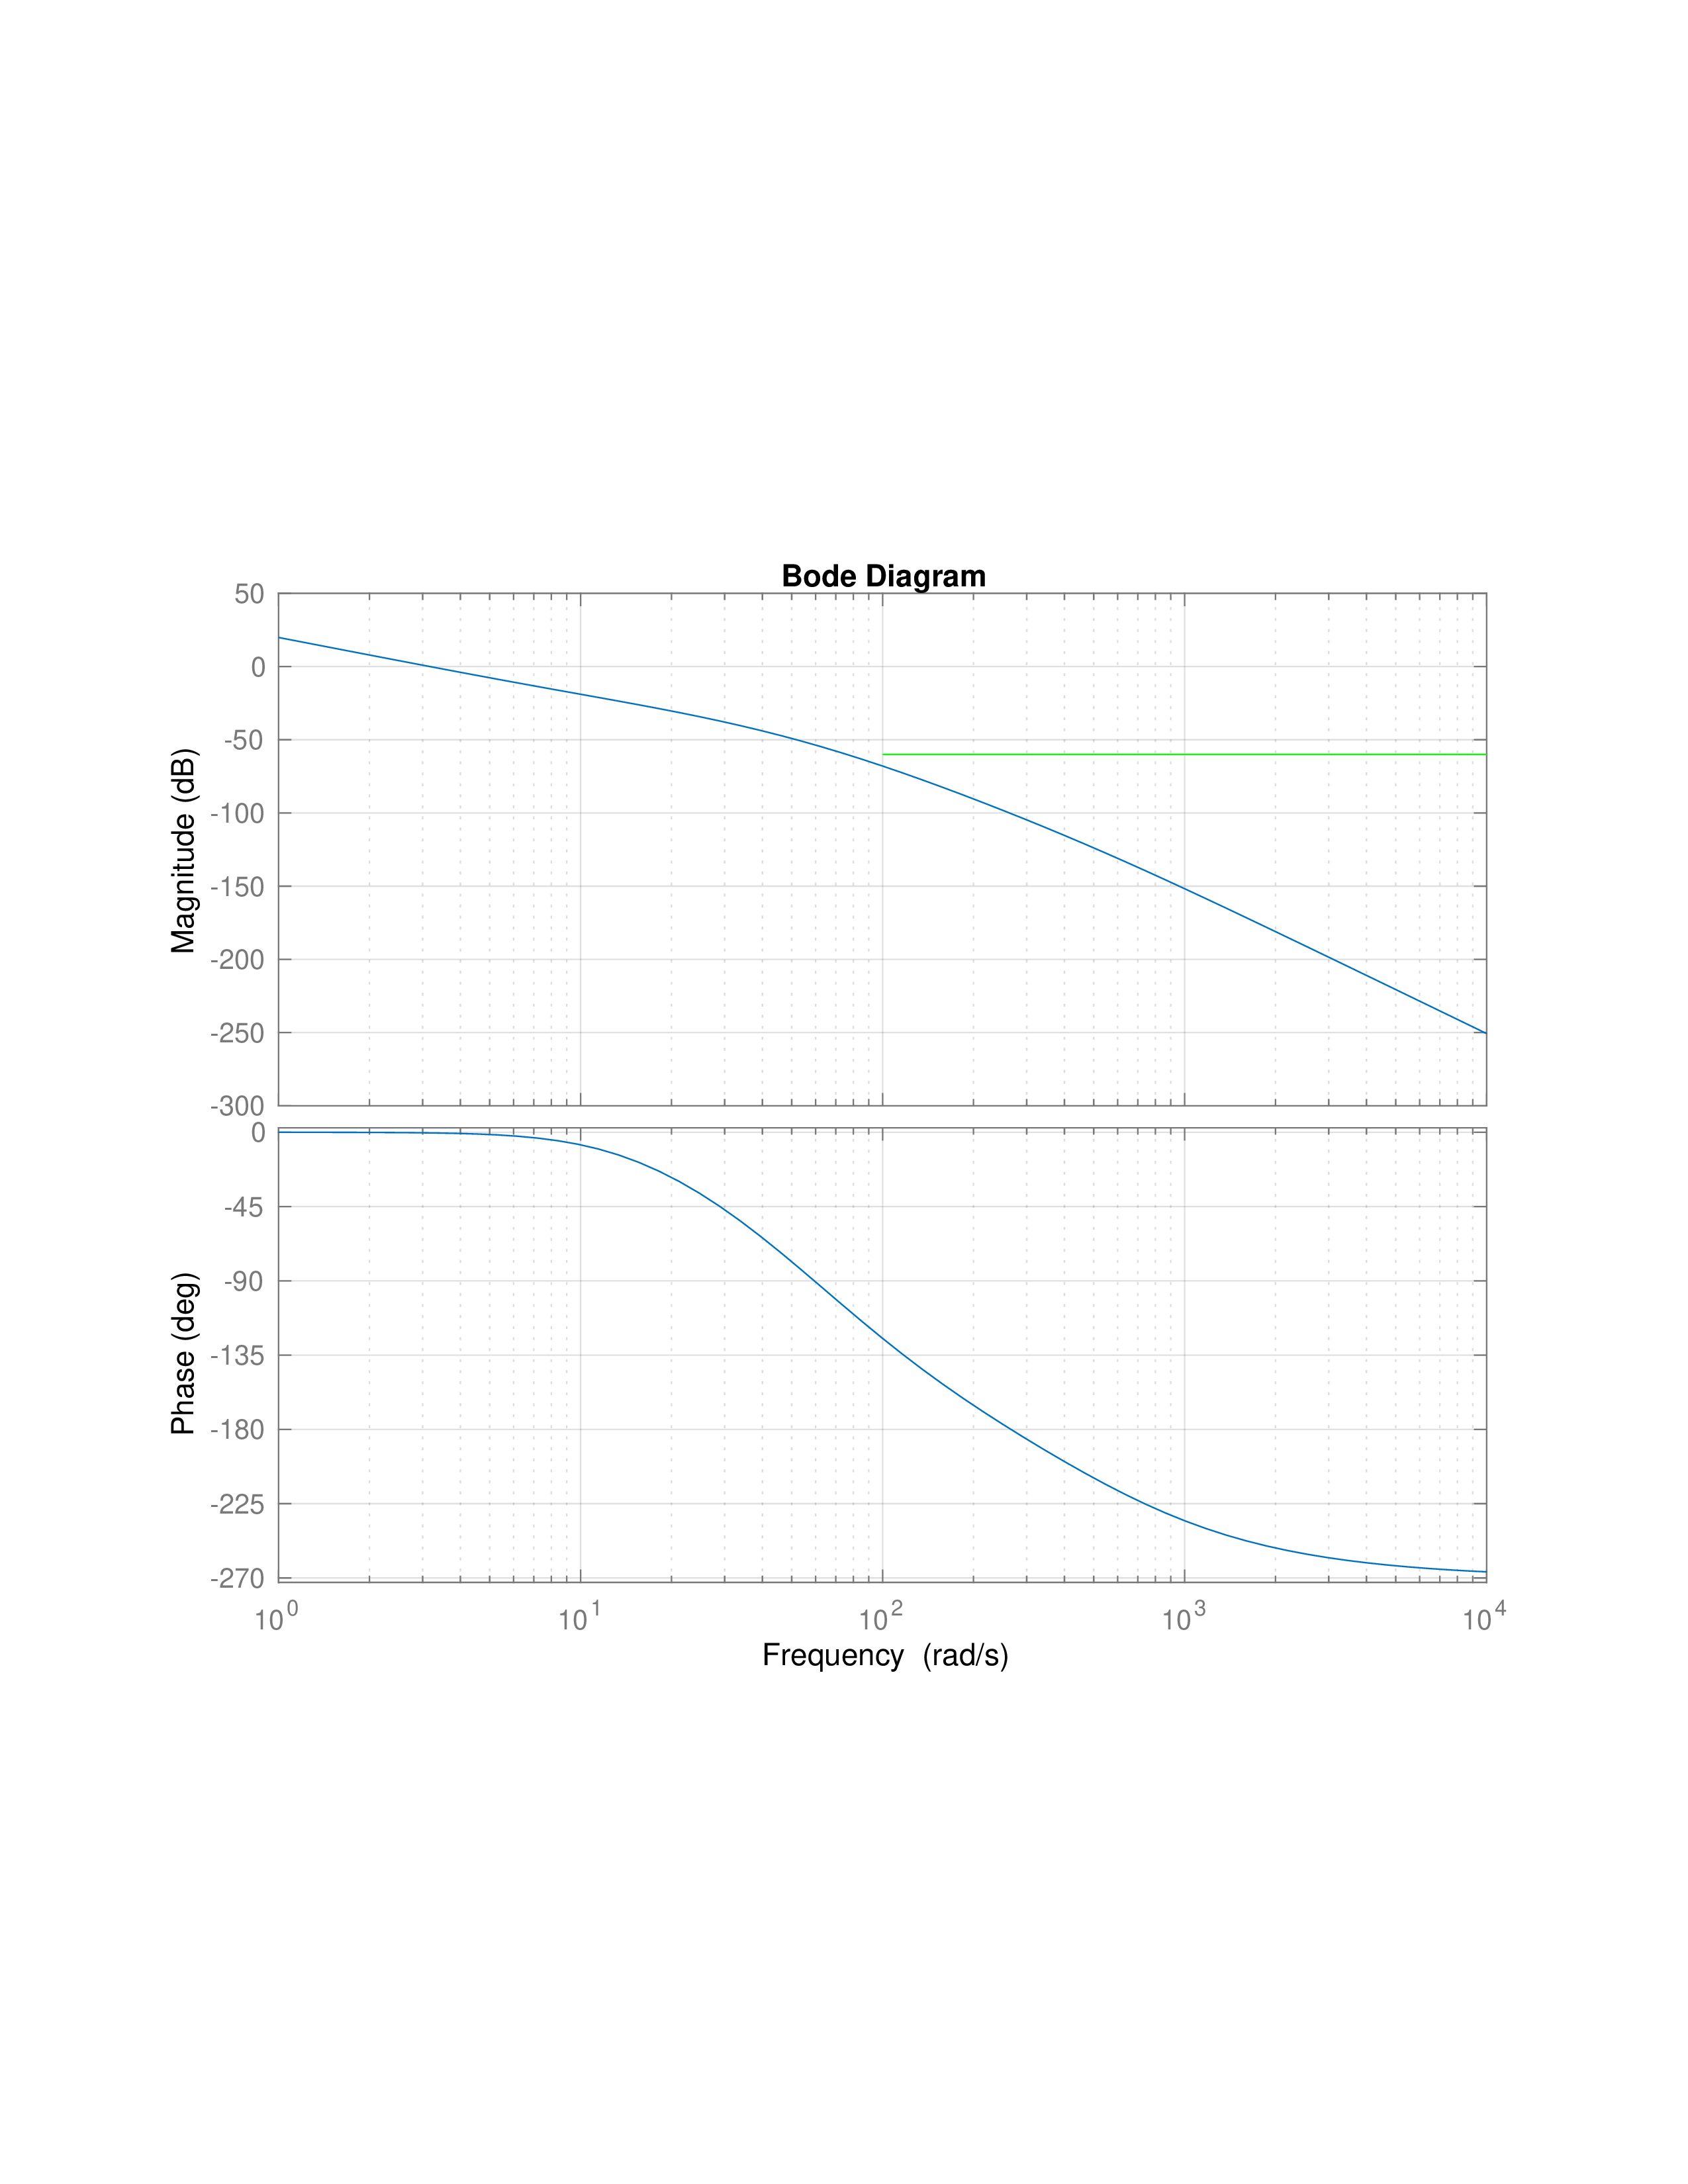
\includegraphics[width=0.95\textwidth]{6_design_studies/figures/hw_ballbeam_compensator_out_design_1.pdf}
   \caption{The Bode plot for the outer loop plant in HW~\ref{hw:ballbeam}.\ref{chap:loopshaping_design}, together with the design specification.}
   \label{fig:hw_ballbeam_compensator_out_design_1}
\end{figure}
The first step is to add a negative proportional gain to lower the bandwidth to reduce the size of the control input.  The result is shown in Figure~\ref{fig:hw_ballbeam_compensator_out_design_2} where $k_p=-0.1$.
\begin{figure}[H]
   \centering
   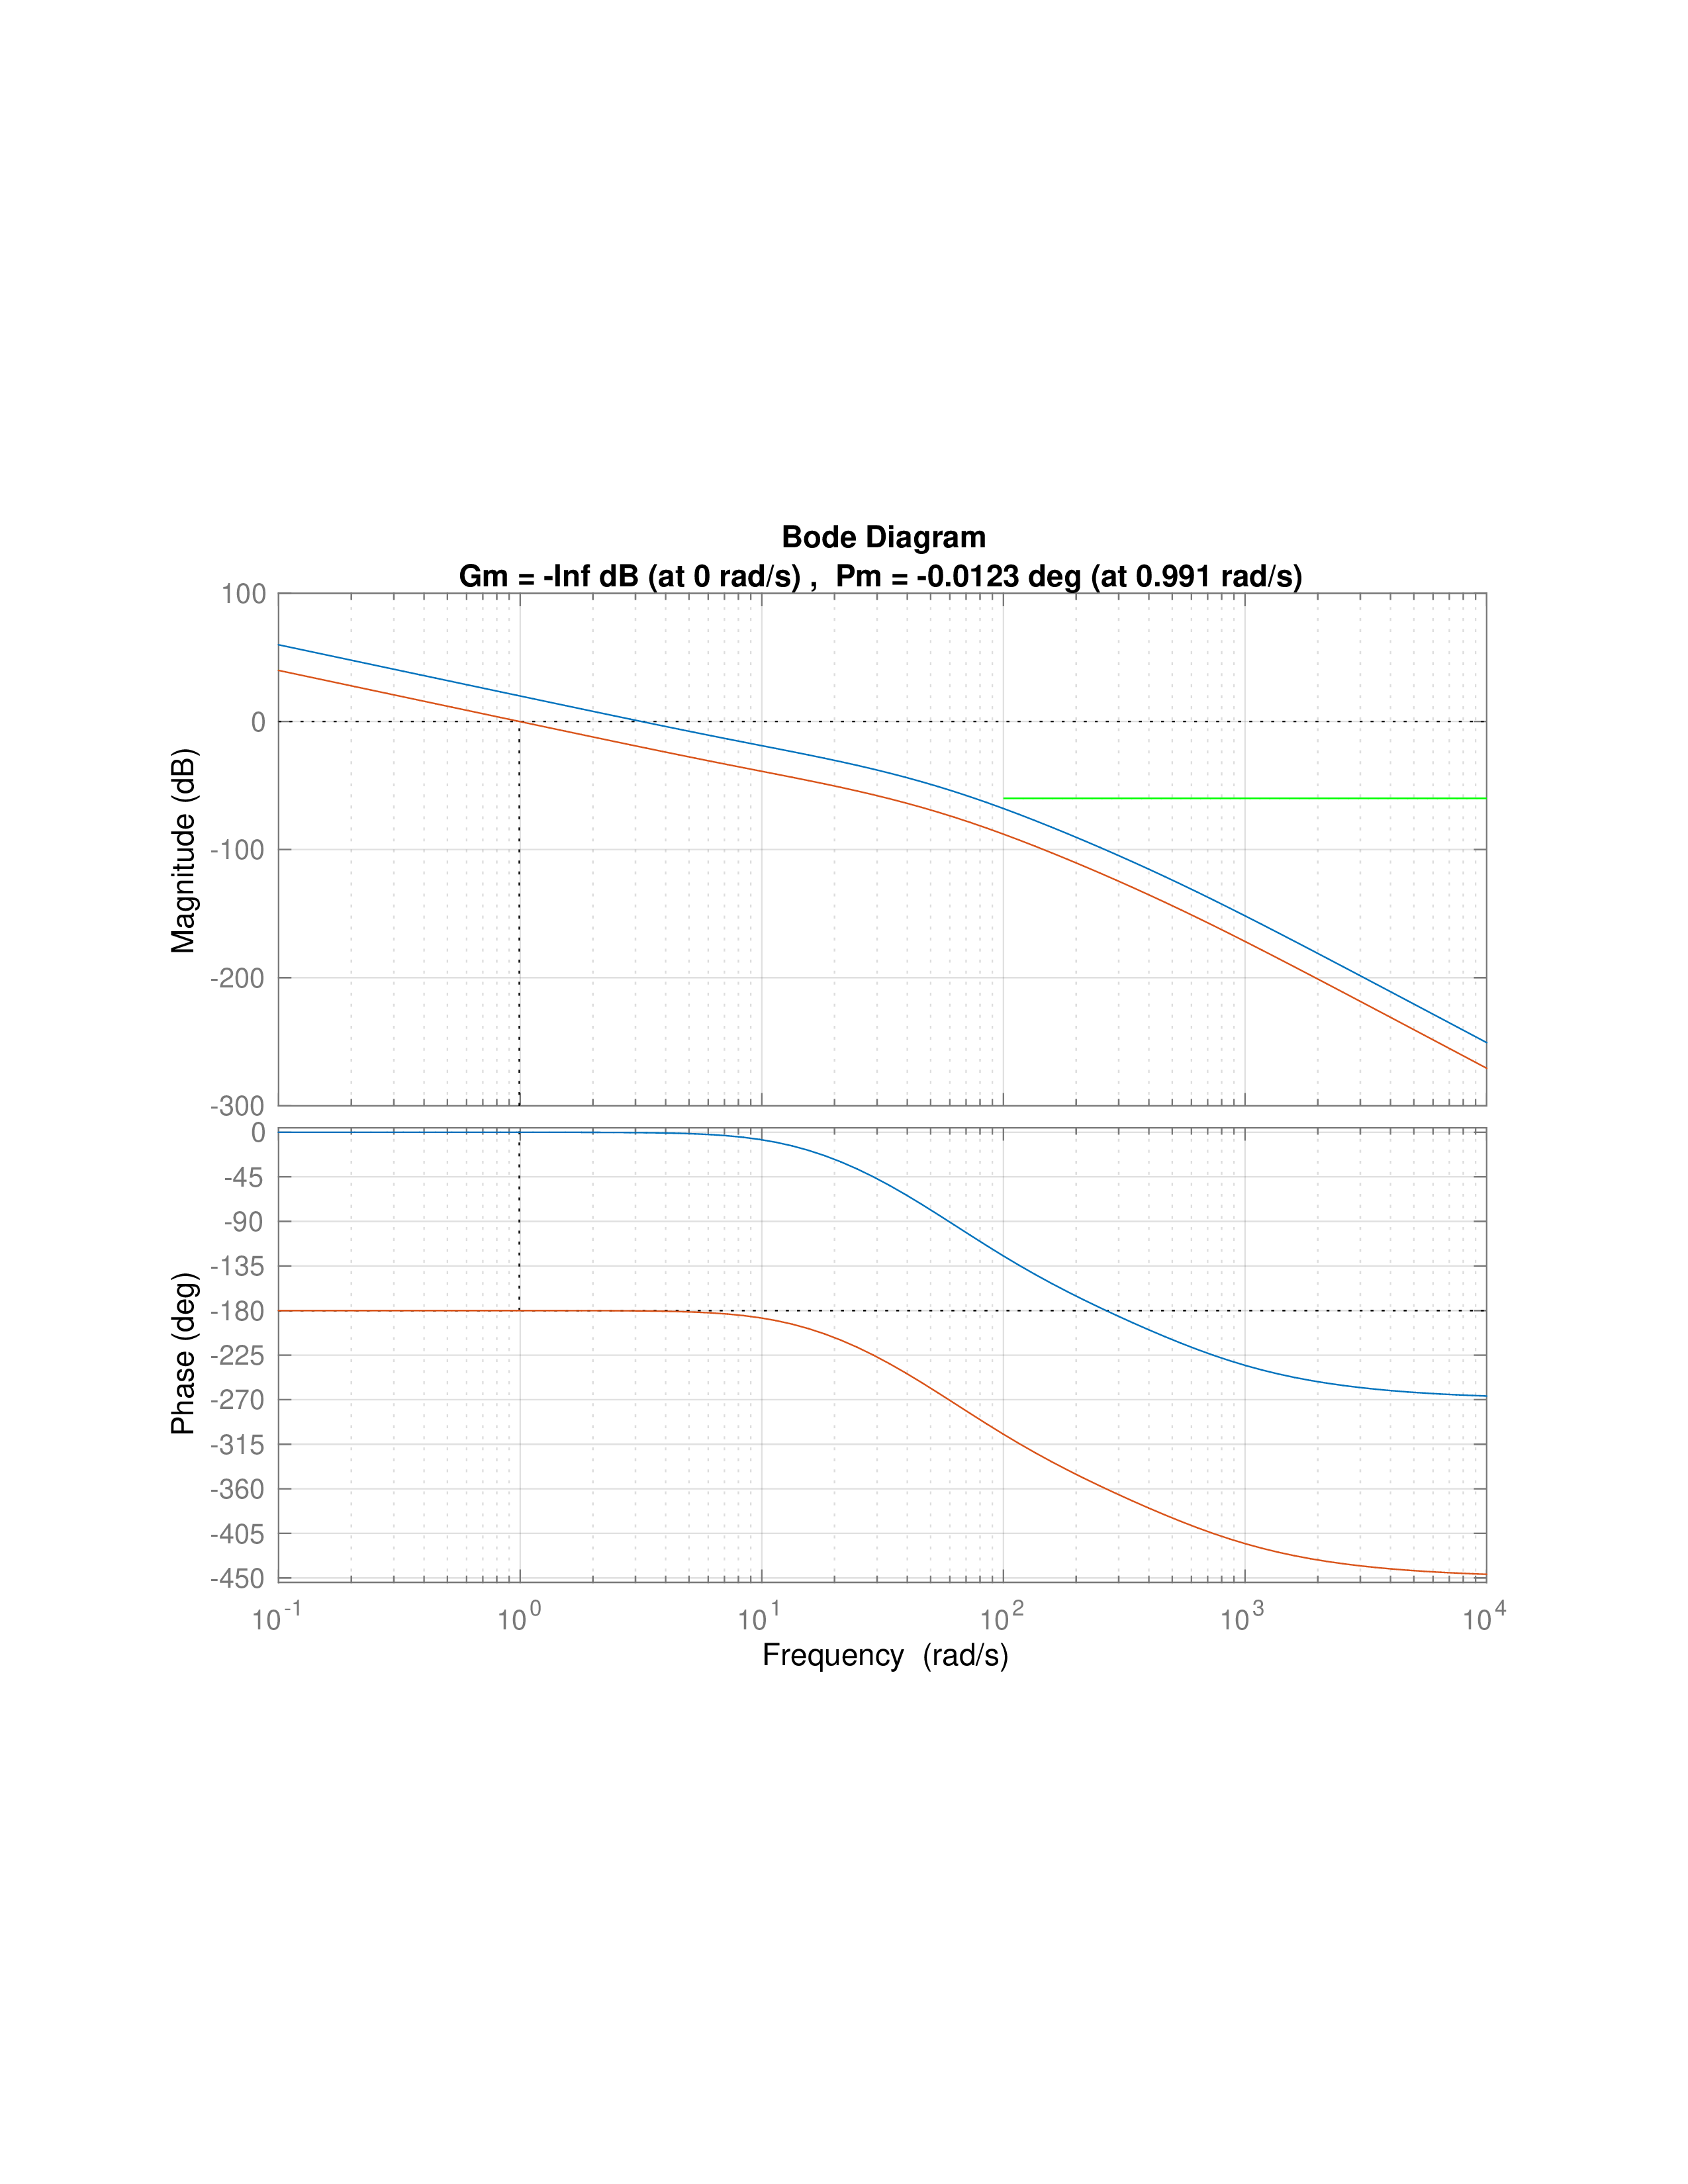
\includegraphics[width=0.95\textwidth]{6_design_studies/figures/hw_ballbeam_compensator_out_design_2.pdf}
   \caption{The Bode plot for the outer loop system in HW~\ref{hw:ballbeam}.\ref{chap:loopshaping_design}, with negative proportional gain.}
   \label{fig:hw_ballbeam_compensator_out_design_2}
\end{figure}
To reject constant input disturbances, integral control is added.  Integral control is also used to satisfy the tracking specification.  
Figure~\ref{fig:hw_ballbeam_compensator_out_design_3}
shows the loopgain after adding
\[
C_{int} = \frac{s+0.3}{s}.
\]
\begin{figure}[H]
   \centering
   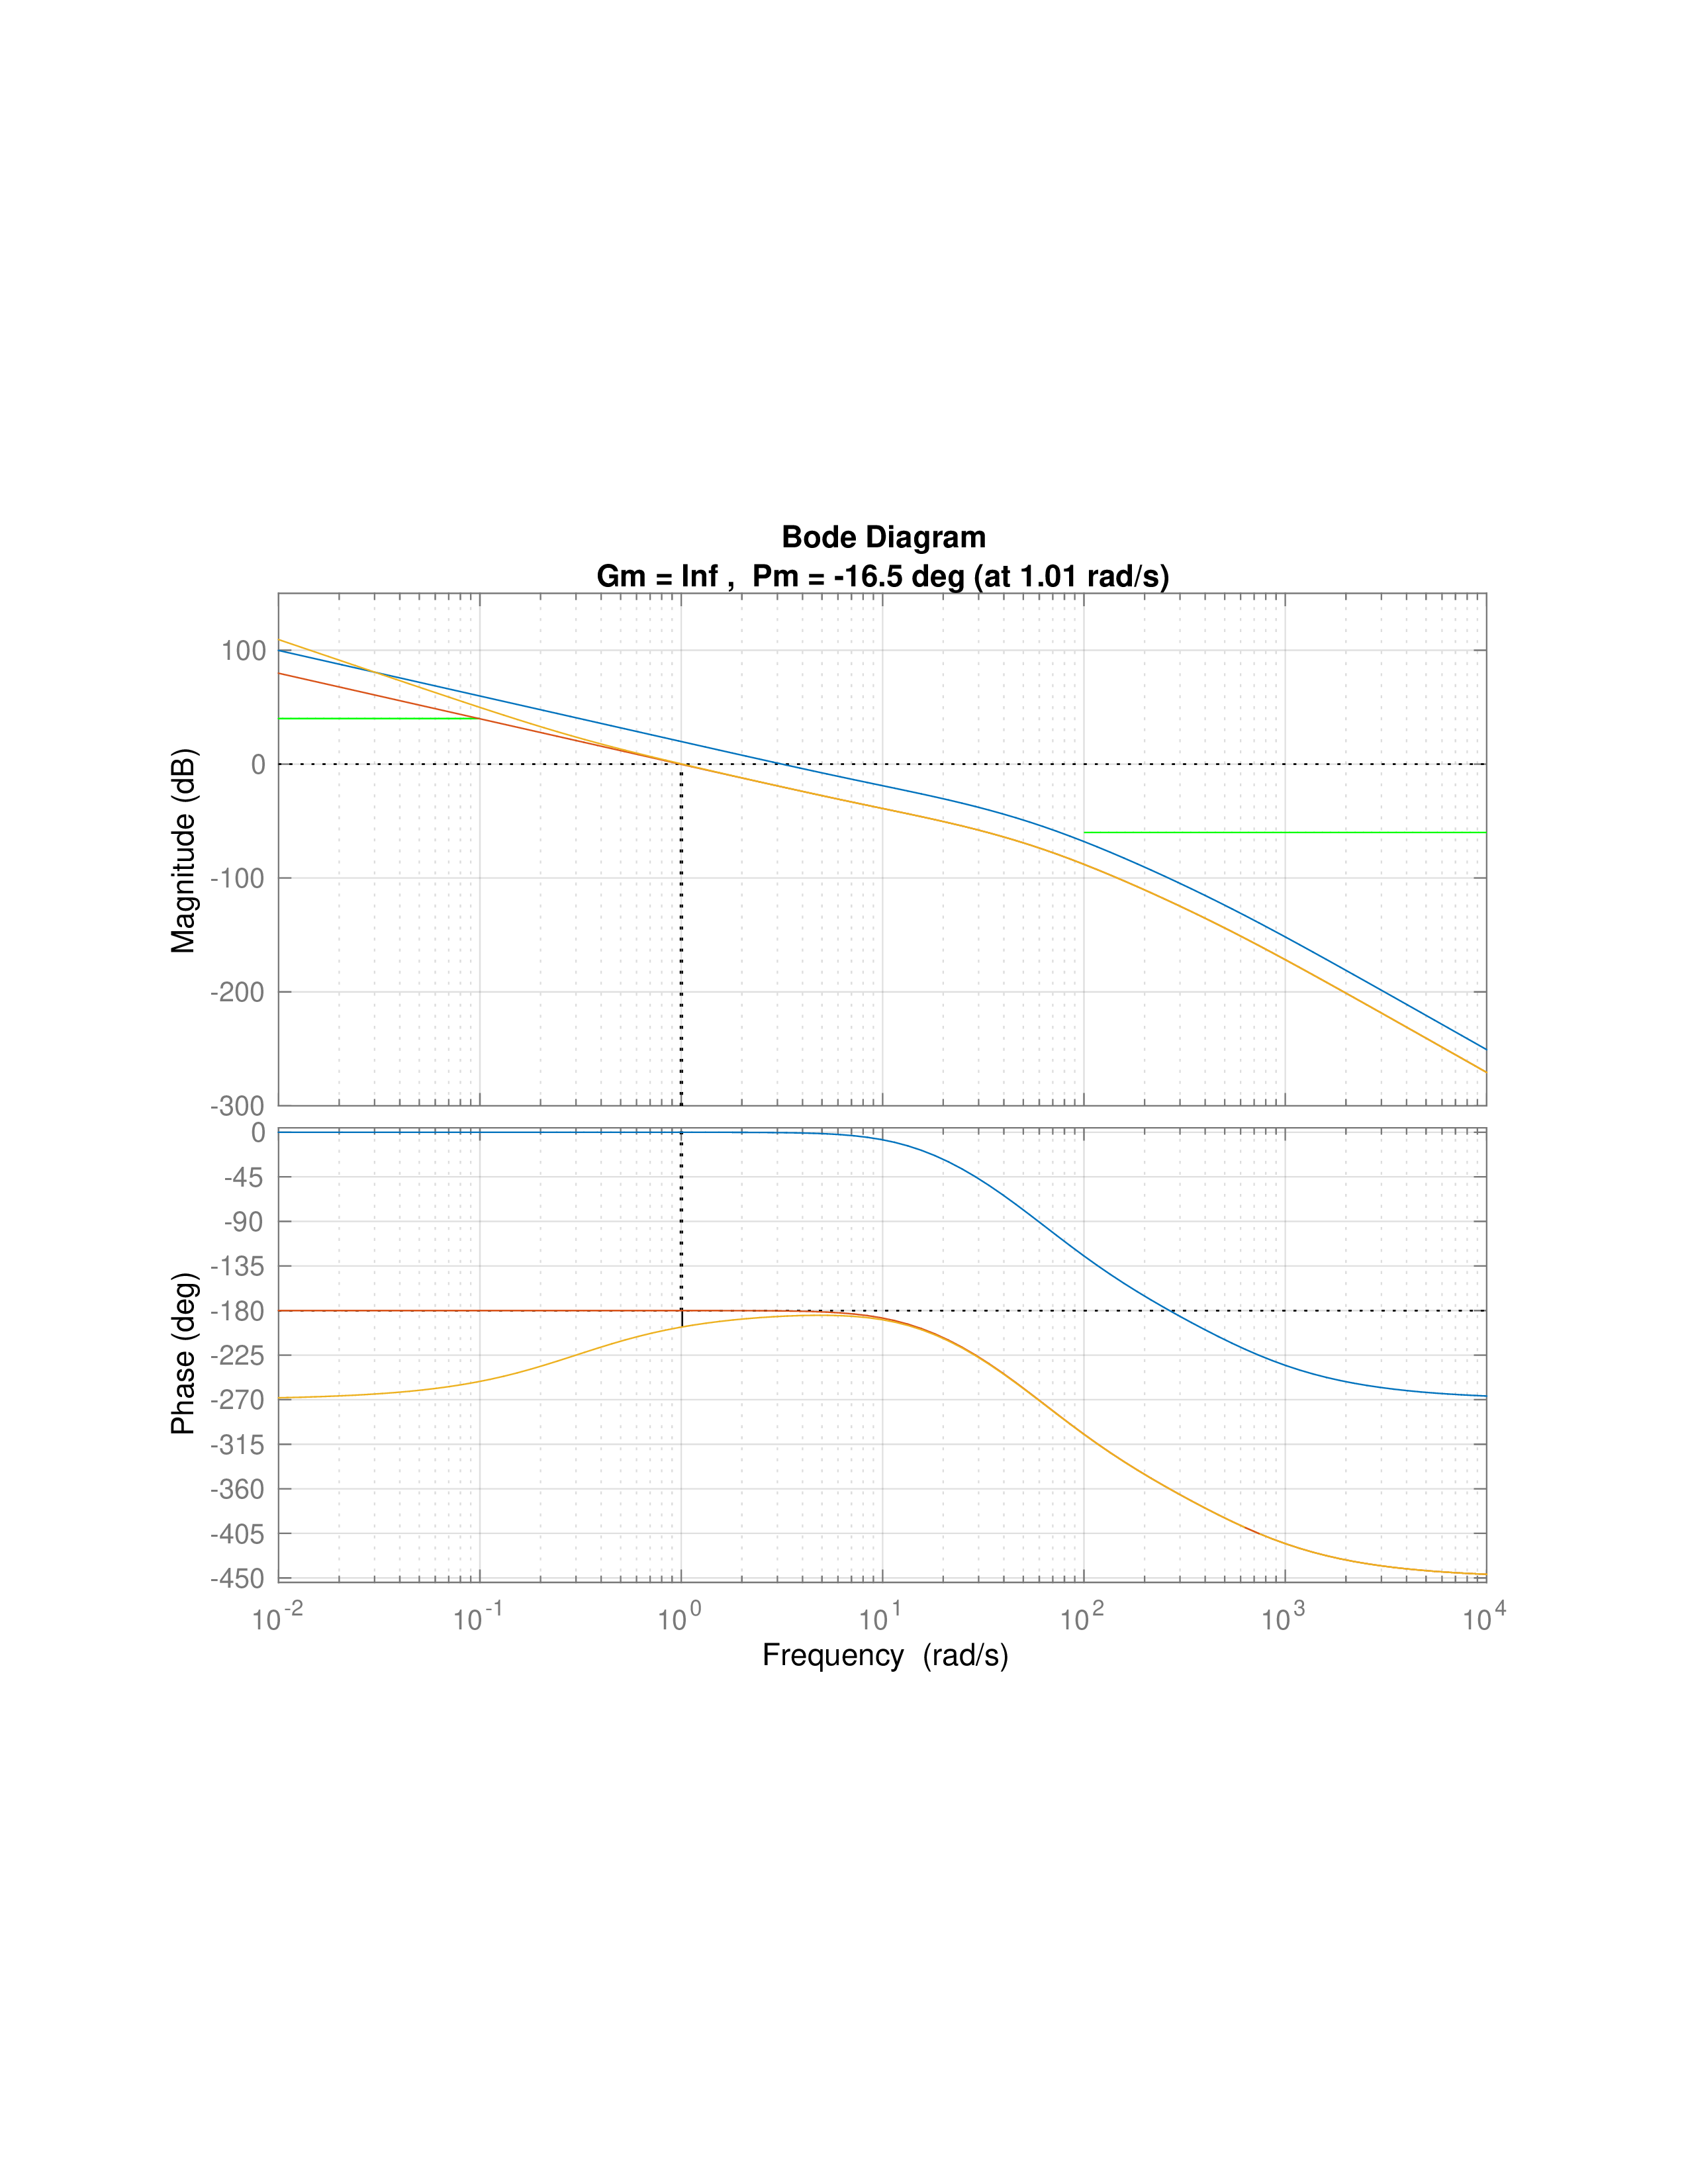
\includegraphics[width=0.95\textwidth]{6_design_studies/figures/hw_ballbeam_compensator_out_design_3.pdf}
   \caption{The Bode plot for the outer loop system in HW~\ref{hw:ballbeam}.\ref{chap:loopshaping_design}, with proportional and integral control.}
   \label{fig:hw_ballbeam_compensator_out_design_3}
\end{figure}
Note that the phase margin is negative which implies that the closed loop system is currently unstable. 
To stabilize the system, a phase lead compensator needs to be added around the cross over frequency.  Figure~\ref{fig:hw_ballbeam_compensator_in_design_4} shows the addition of the phase lead filter
\[
C_{lead} = \frac{25(s+\frac{2}{\sqrt{25}})}{(s+\frac{2}{\sqrt{25}})},
\]
which results in a phase margin of $PM=59.8$~degrees.
\begin{figure}[H]
   \centering
   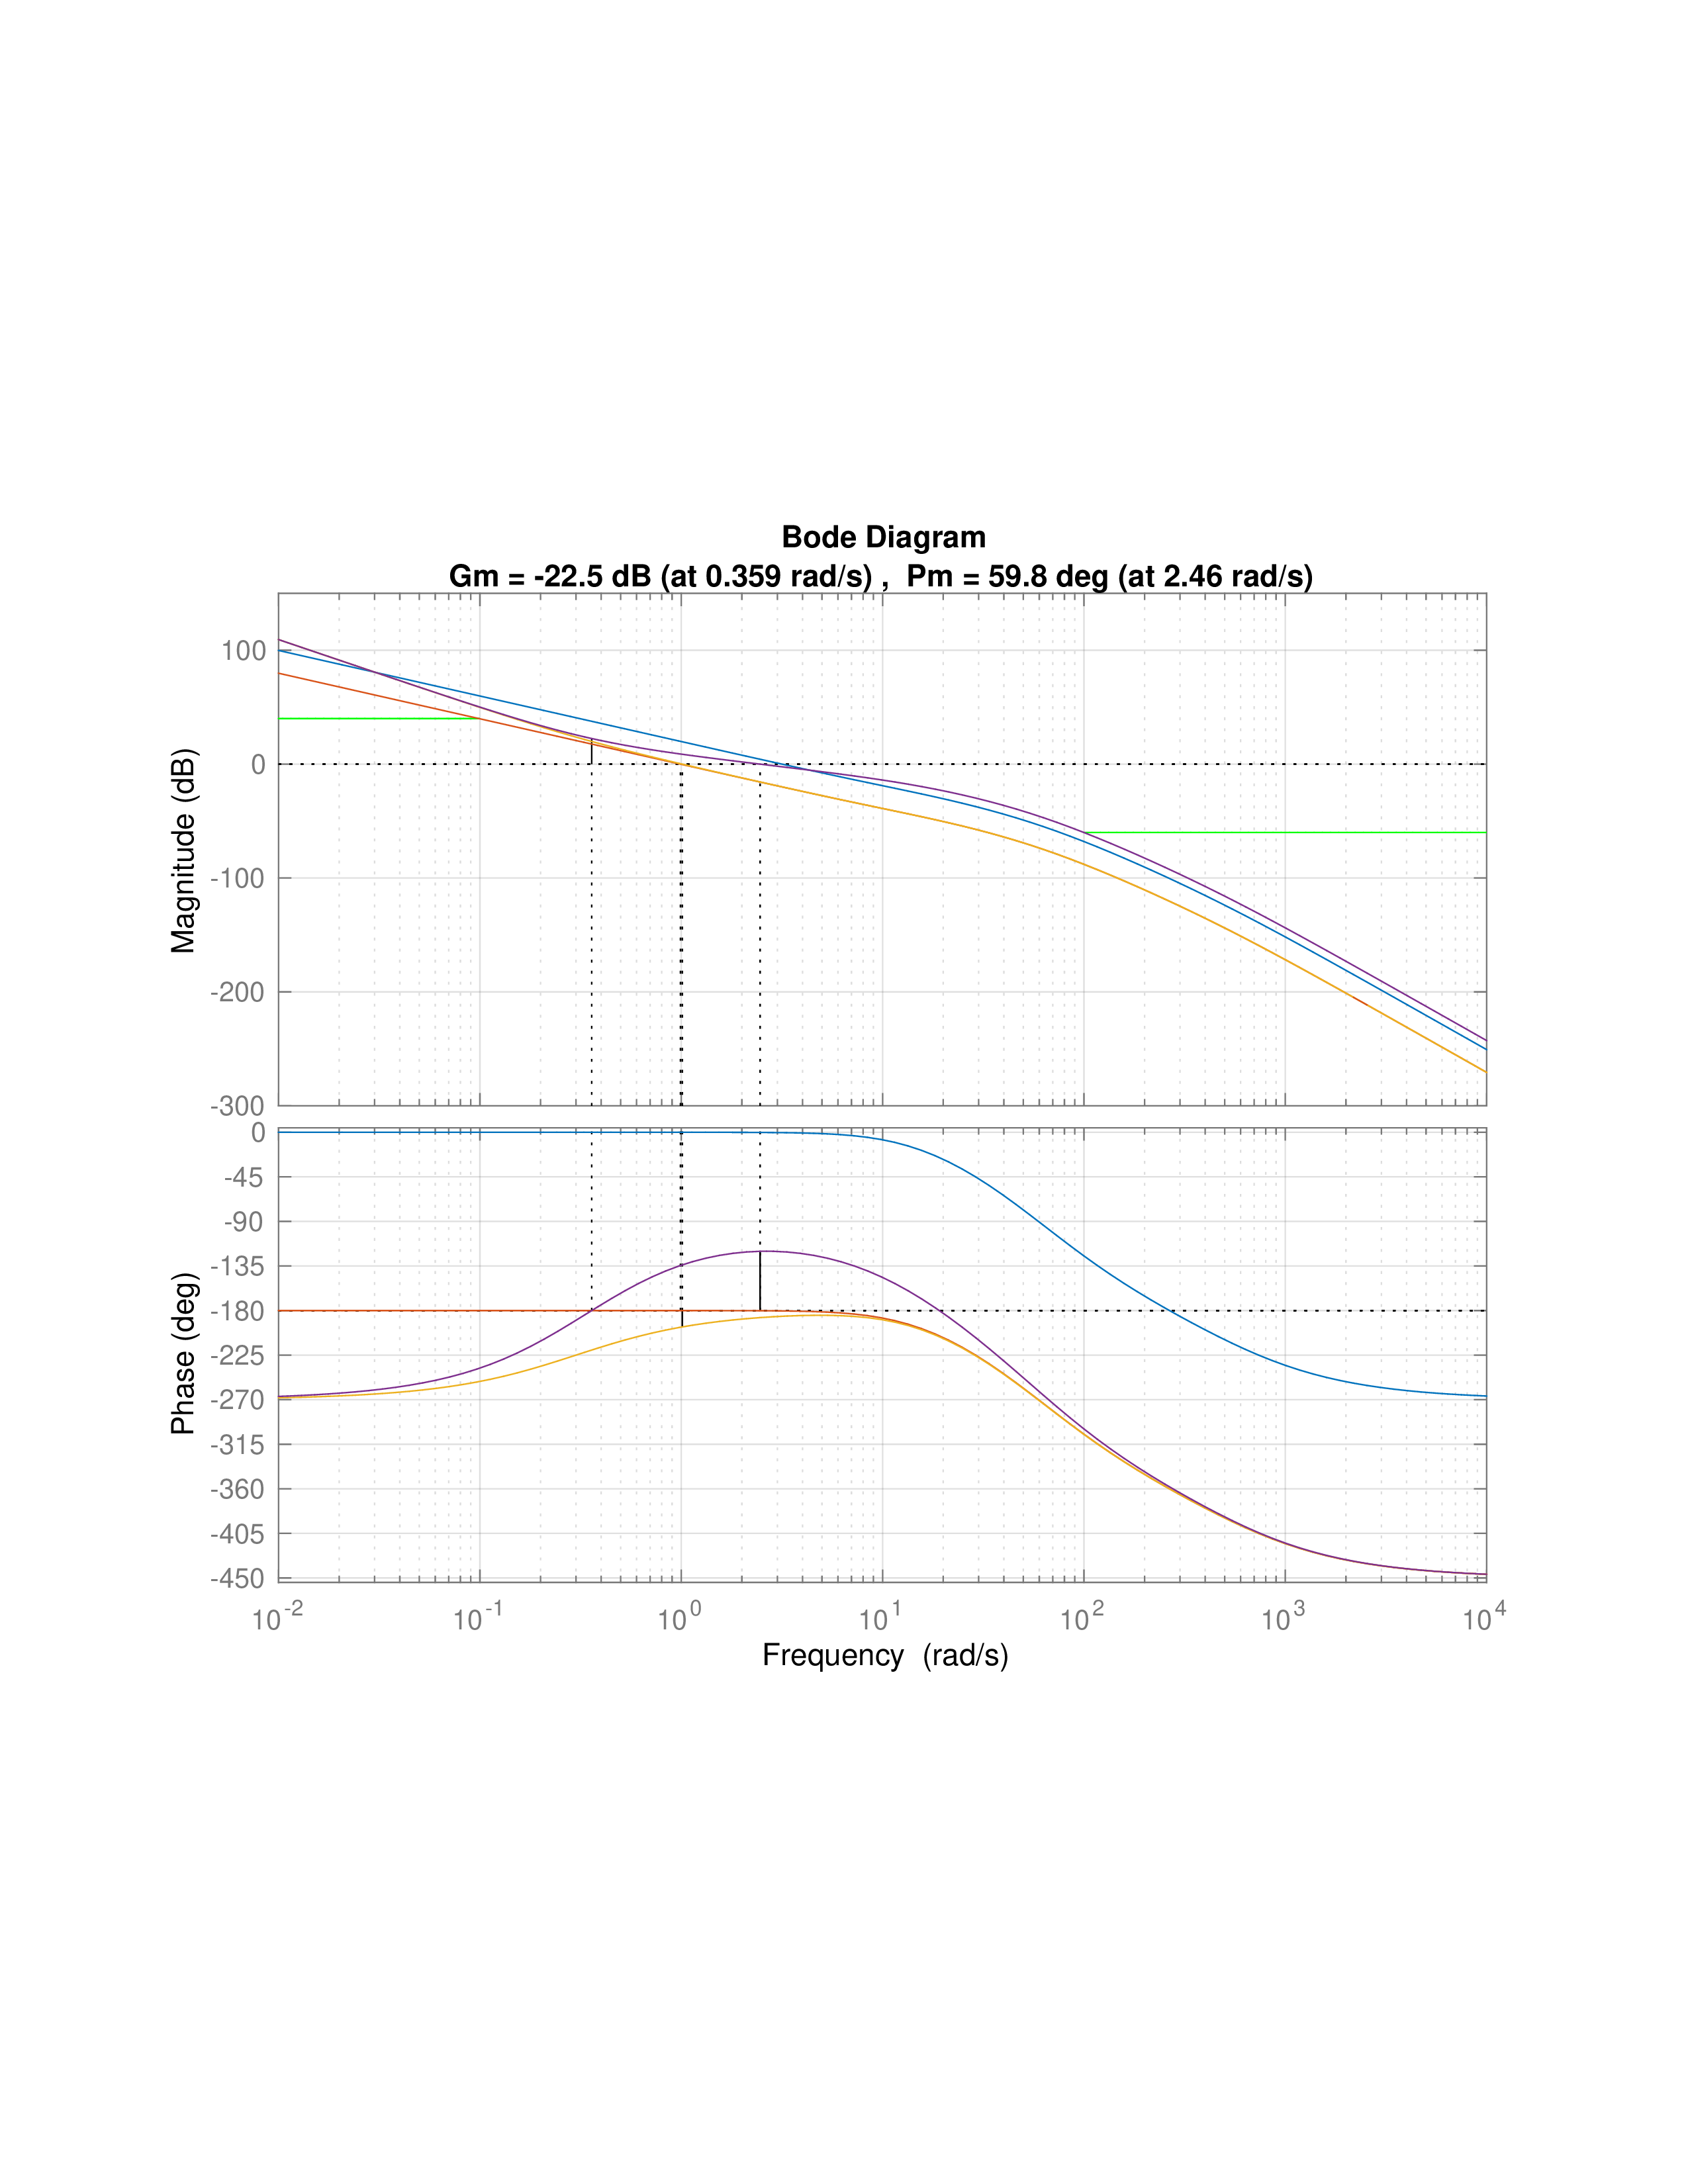
\includegraphics[width=0.95\textwidth]{6_design_studies/figures/hw_ballbeam_compensator_out_design_4.pdf}
   \caption{The Bode plot for the outer loop system in HW~\ref{hw:ballbeam}.\ref{chap:loopshaping_design}, with proportional gain, integral control, and phase lead compensation.}
   \label{fig:hw_ballbeam_compensator_out_design_4}
\end{figure}
To meet the noise specification, the low pass filter
\[
C_{lpf} = \frac{50}{s+50}
\]
is added to the compensator, and the resulting loopgain is shown in Figure~\ref{fig:hw_ballbeam_compensator_out_design_5}.
\begin{figure}[H]
   \centering
   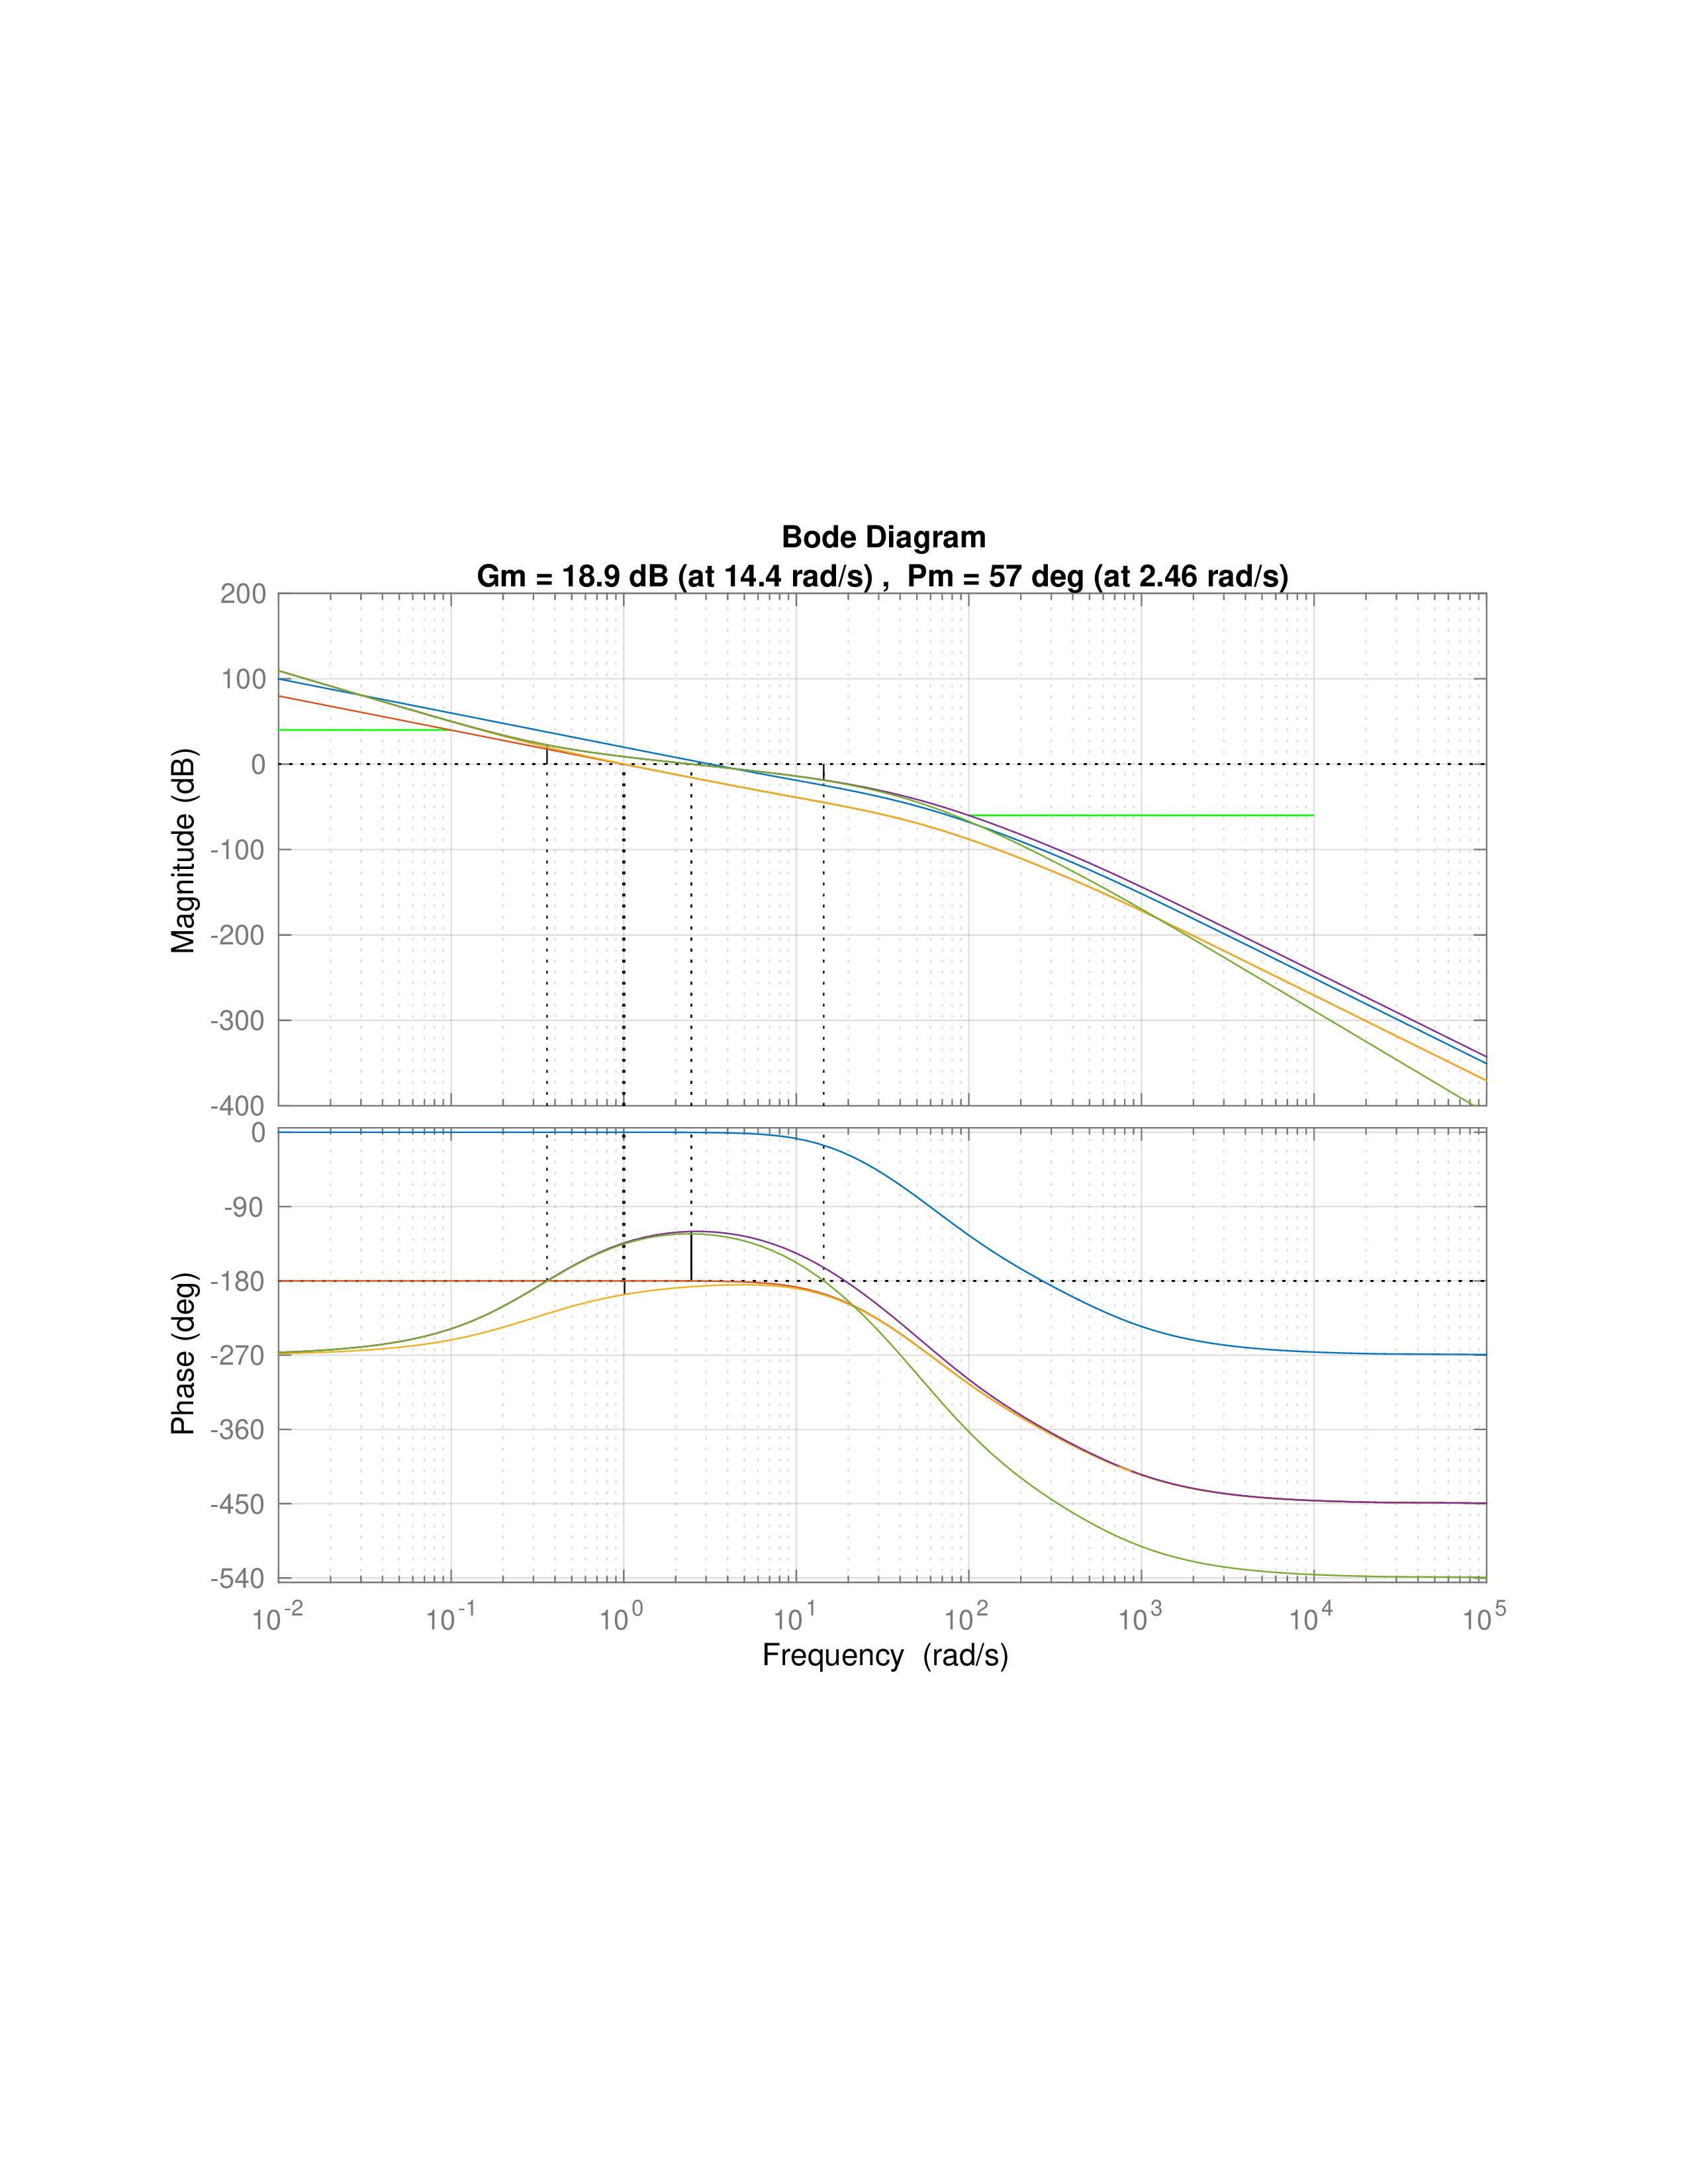
\includegraphics[width=0.95\textwidth]{6_design_studies/figures/hw_ballbeam_compensator_out_design_5.pdf}
   \caption{The Bode plot for the outer loop system in HW~\ref{hw:ballbeam}.\ref{chap:loopshaping_design}, with proportional gain, integral control, phase lead compensation, and a low pass  filter.}
   \label{fig:hw_ballbeam_compensator_out_design_5}
\end{figure}
The resulting compensator is
\[
C_{out}(s) = -0.1\left(\frac{s+0.3}{s}\right)\left(\frac{25(s+\frac{2}{\sqrt{25}})}{(s+\frac{2}{\sqrt{25}})}\right)\left(\frac{50}{s+50}\right).
\]
The closed loop response for both the inner and outer loop systems, 
as well as the unit step response for the output and control signal of the outer loops are all show in Figure~\ref{fig:hw_ballbeam_compensator_out_design_6}.
\begin{figure}[H]
   \centering
   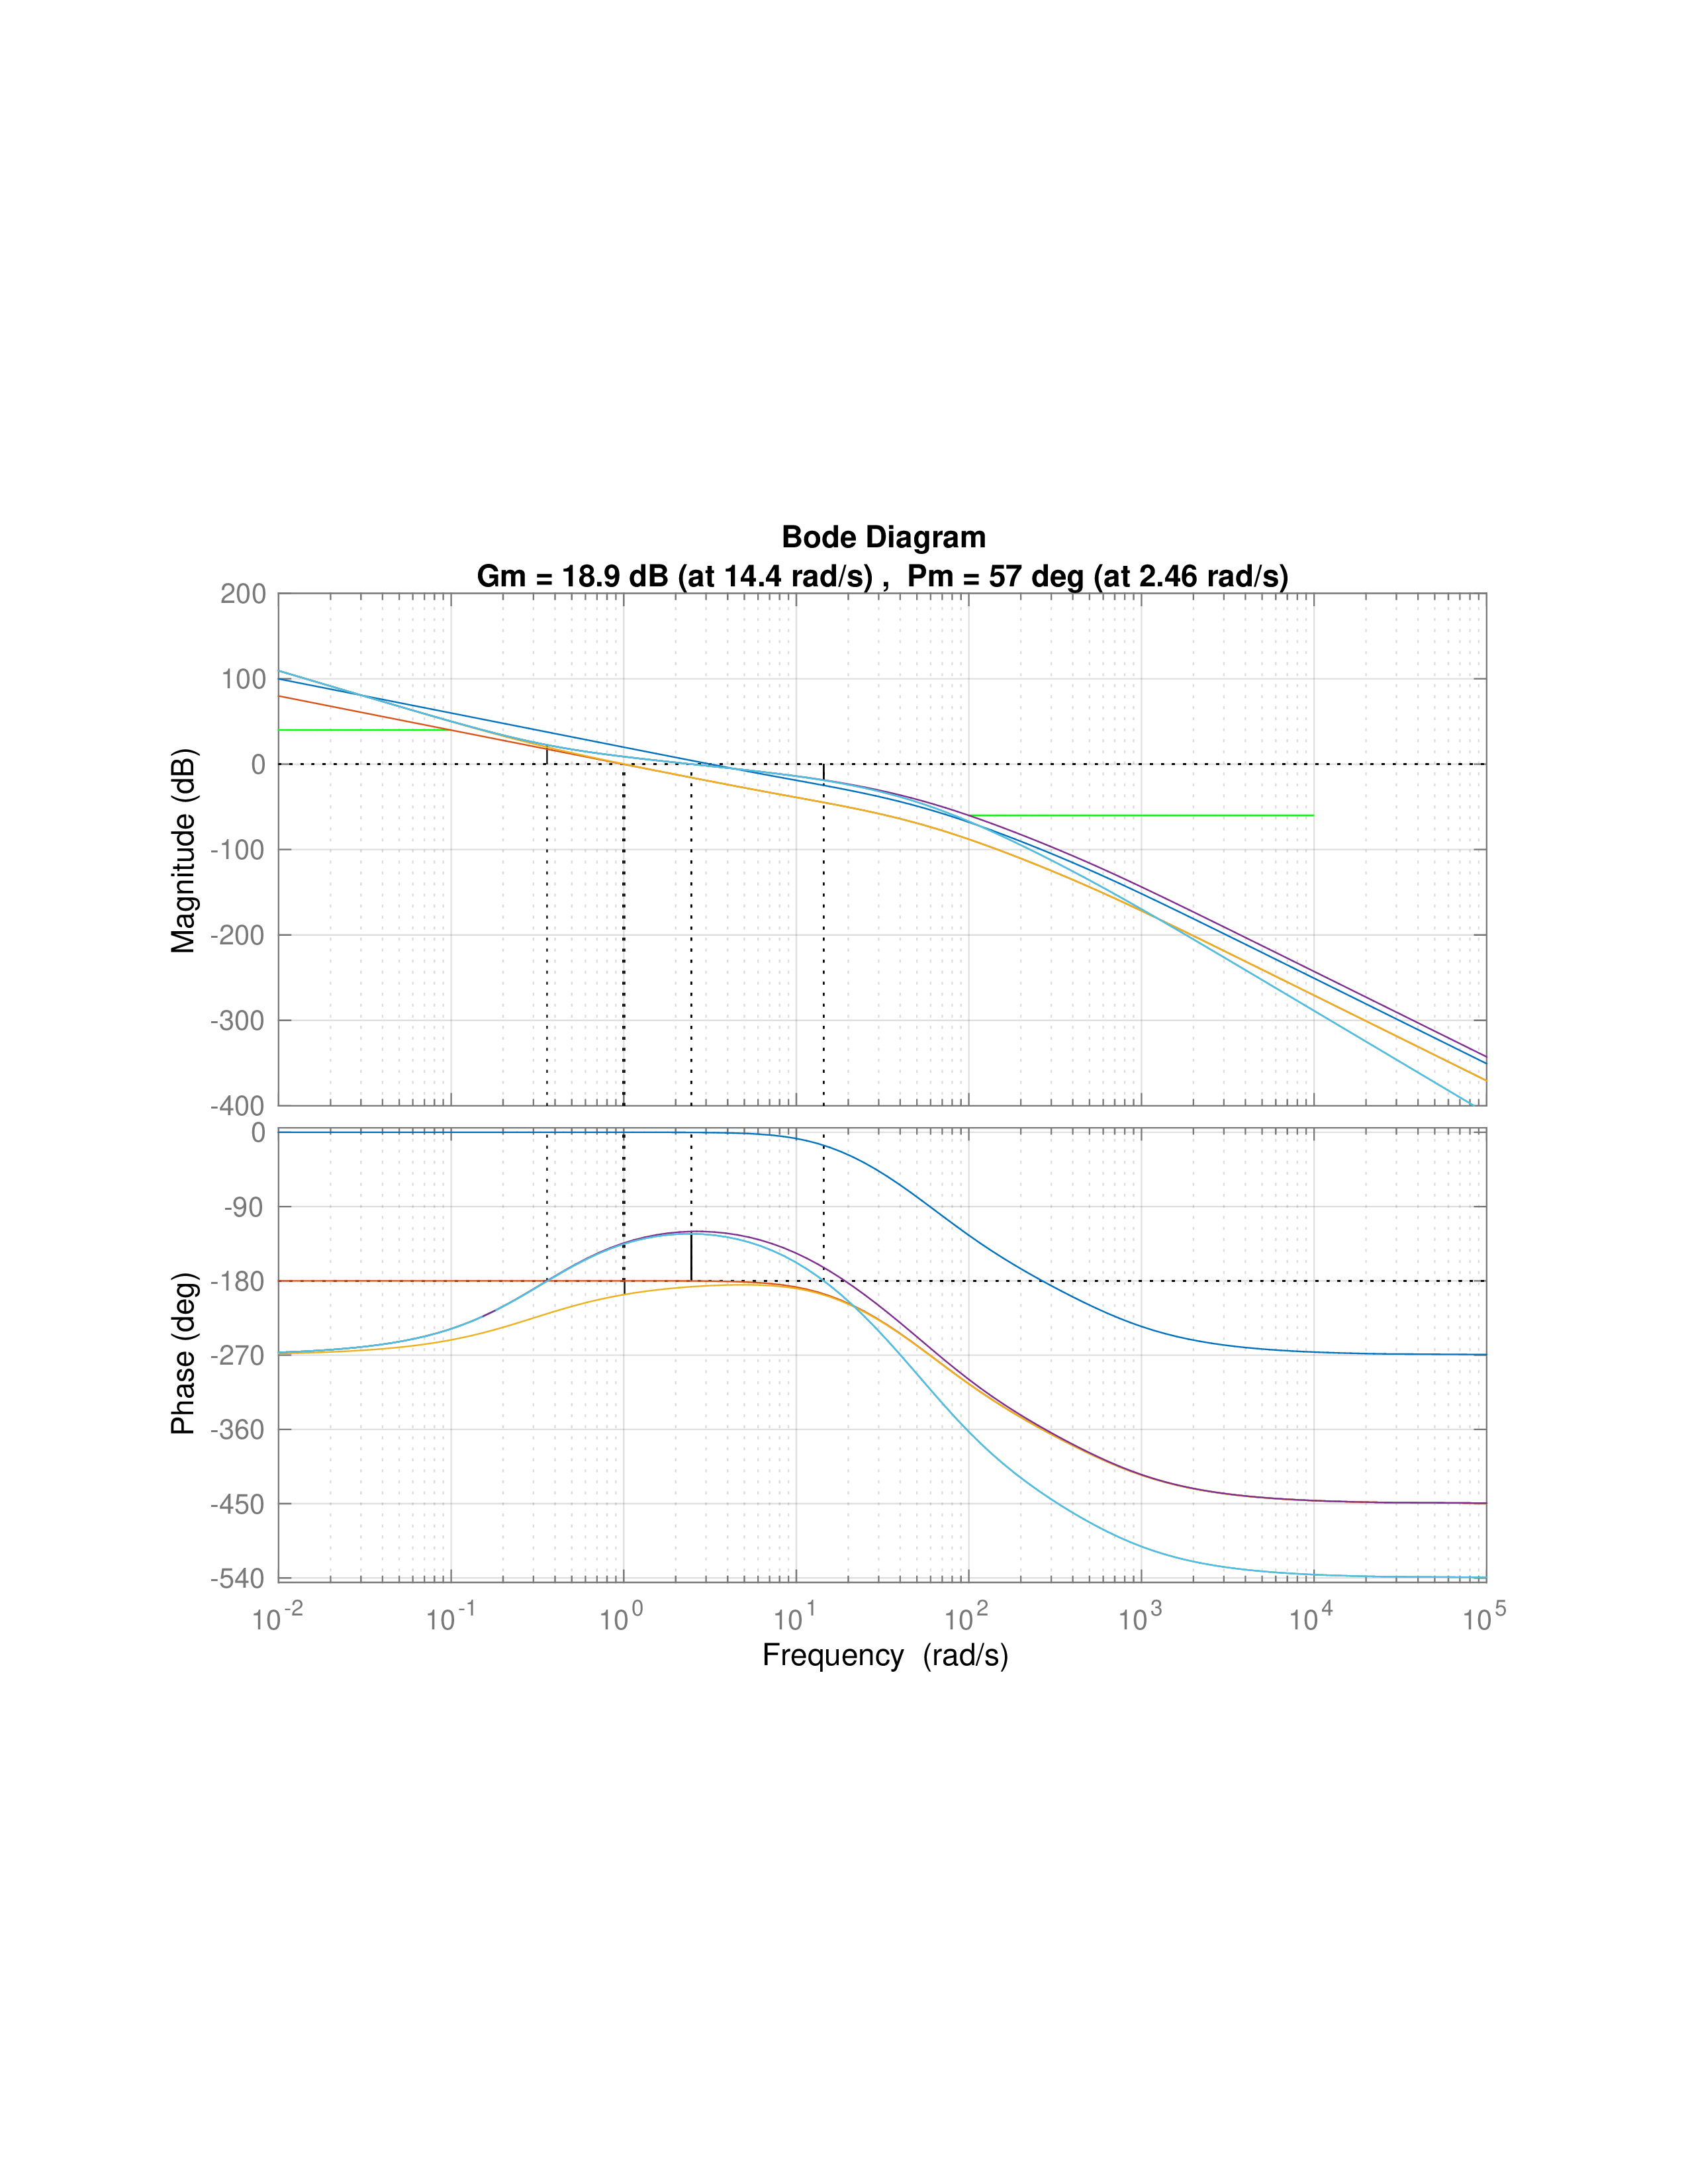
\includegraphics[width=0.95\textwidth]{6_design_studies/figures/hw_ballbeam_compensator_out_design_6.pdf}
   \caption{The closed loop bode response, the unit step response for the output, and the unit step response for the input of the inner loop design in HW~\ref{hw:ballbeam}.\ref{chap:loopshaping_design}.}
   \label{fig:hw_ballbeam_compensator_out_design_6}
\end{figure}

The Matlab code used to design the outer loop is shown below.
\begin{lstlisting}
Plant = minreal(P_out*(P_in*C_in/(1+P_in*C_in)));

%%%%%%%%%%%%%%%%%%%%%%%%%%%%%%%%%%%%%%%%%%%%%%%%%%%%%%%%%%%
%  Define Design Specifications
%%%%%%%%%%%%%%%%%%%%%%%%%%%%%%%%%%%%%%%%%%%%%%%%%%%%%%%%%%%

%--- general tracking specification ---
    omega_r = 10^-1;  % track signals below this frequency
    gamma_r = 10^(-40/20);  % tracking error below this value
    w = logspace(log10(omega_r)-2,log10(omega_r));

    %--- noise specification ---
    omega_n = 10^2;  % attenuate noise above this frequency
    gamma_n = 10^(-60/20);   % attenuate noise by this amount
    w = logspace(log10(omega_n),2+log10(omega_n));

%%%%%%%%%%%%%%%%%%%%%%%%%%%%%%%%%%%%%%%%%%%%%%%%%%%%%%%%%%%
% Control Design
  C = tf(1,1);
%%%%%%%%%%%%%%%%%%%%%%%%%%%%%%%%%%%%%%%%%%%%%%%%%%%%%%%%%%%

% proportional control: change cross over frequency
     kp = -0.1;
     C = C*kp;

% integral control: increase steady state tracking and dist rejection
     k_I = .3; % frequency at which integral action ends
     Integrator = tf([1,k_I],[1,0]);
     C = C*Integrator;

% phase lead: increase PM (stability)
    wmax = 2; % location of maximum frequency bump
    M    = 25; % separation between zero and pole
    Lead =tf(M*[1,wmax/sqrt(M)],[1,wmax*sqrt(M)]);
    C = C*Lead;

% low pass filter: decrease gain at high frequency (noise)
     p = 50;
     LPF = tf(p,[1,p]);
     C = C*LPF;

%%%%%%%%%%%%%%%%%%%%%%%%%%%%%%%%%%%%%%%%%%%%%%%%%%%%%%%%%%%
% Prefilter Design
  F = tf([1],[1]);
%%%%%%%%%%%%%%%%%%%%%%%%%%%%%%%%%%%%%%%%%%%%%%%%%%%%%%%%%%%

% low pass filter
    p = 1;  % frequency to start the LPF
    LPF = tf(p, [1,p]);
    F = F*LPF;

        
%%%%%%%%%%%%%%%%%%%%%%%%%%%%%%%%%%%%%%%%%%%%%%%%%%%%%%%%%%%% Convert controller to state space equations 
%%%%%%%%%%%%%%%%%%%%%%%%%%%%%%%%%%%%%%%%%%%%%%%%%%%%%%%%%%%%
C=minreal(C);
[num,den] = tfdata(C,'v');
[P.Aout_C,P.Bout_C,P.Cout_C,P.Dout_C]=tf2ss(num,den);

[num,den] = tfdata(F,'v');
[P.Aout_F, P.Bout_F, P.Cout_F, P.Dout_F] = tf2ss(num,den);

C_out=C;
\end{lstlisting}

The complete Simulink files are on the wiki associated with the book.



